\documentclass[11pt]{article}
\usepackage[margin = 1in]{geometry}

\usepackage{amssymb}
\usepackage{afterpage}
\usepackage{array}
\usepackage{url}
\usepackage{natbib}
\usepackage[capposition=top]{floatrow}

\input{"paper_header"}
\graphicspath{{"figures/"}}

\renewenvironment{abstract}
 {\small
  \begin{center}
  \bfseries \abstractname\vspace{-.5em}\vspace{0pt}
  \end{center}
  \list{}{
    \setlength{\leftmargin}{35mm}
    \setlength{\rightmargin}{\leftmargin}%
  }
  \item\relax}
 {\endlist}

 \usepackage[dvipsnames]{xcolor}
 \usepackage{adjustbox}

%--------------------------------------------------------------
% Misc formatting
%--------------------------------------------------------------

\newcommand{\red}[1]{\textcolor{red}{#1}}
\newcommand{\blue}[1]{\textcolor{blue}{#1}}
\newcommand{\orange}[1]{\textcolor{orange}{#1}}
\newcommand{\violet}[1]{\textcolor{violet}{#1}}
\newcommand{\var}[1]{\textcolor{internationalkleinblue}{\texttt{#1}}}
\newcommand{\zvar}[1]{\textcolor{dgreen}{\texttt{#1}}}

% COMMENT OUT TO MAKE BLACK
%\definecolor{red}{cmyk}{0,0,0,1}
%\definecolor{blue}{cmyk}{0,0,0,1}
%\definecolor{orange}{cmyk}{0,0,0,1}
%\definecolor{violet}{cmyk}{0,0,0,1}

\usepackage{times}
%\usepackage{helvet}
%\renewcommand{\familydefault}{\sfdefault}
\doublespacing
\emergencystretch 3em




%--------------------------------------------------------------
% Information
%--------------------------------------------------------------

\newcommand{\titletext}{Harnessing Social Media Influencers (or Simply Using Ads?)}

\newcommand{\authors}{
	Antonella Bandiera\thanks{Assistant Professor, Department of Political Science, ITAM. antonella.bandiera@itam.mx.} \and
    Shelley Liu\footnote{Assistant Professor, Sanford School of Public Policy, Duke University. Email: \href{mailto:shelley.liu@duke.edu}{shelleyxliu@berkeley.edu}} \and 
	Jeremy Bowles\thanks{Assistant Professor, Department of Political Science and School of Public Policy, University College London. jeremy.bowles@ucl.ac.uk.} \and 
	Horacio Larreguy\thanks{Associate Professor, Economics and Political Science, ITAM. horacio.larreguy@itam.mx.} \and
	John Marshall\thanks{Associate Professor, Department of Political Science, Columbia University. jm4401@columbia.edu.} \and
    Eduardo Zago\thanks{PhD Student in Politics, NYU. ez2490@nyu.edu .} \and 
    Joaquín Barrutia\thanks{PhD Student in Economics, Emory University. joaquin.barrutia.alvarez@emory.com.}, 
 
}

\newcommand{\acknowledgements}{}


\newcommand{\abstracttext}{%
	\begin{abstract}
		\noindent 

  
		\\ \vspace{2em}
		
	\end{abstract}
}

\newcommand{\Nintensive}{N = 170,547. }

\newcommand{\Nextensive}{N = 96,390. }

\newcommand{\IntensiveTreatment}{The treatment variable is the number of treated influencers each user follows. We use total influencers followed, treatment and control, fixed effects. Standard errors are estimated using bootstrap repetitions of 1000 different treatment assignments. }

\newcommand{\ExtensiveTreatment}{The treatment variable is a dummy which is 1 if a user follows a treatment influencer, 0 in other case. We use influencer-block fixed effects. Standard errors are estimated using bootstrap repetitions of 1000 different treatment assignments. }

\newcommand{\TreatmentAds}{The treatment variable is 1 for users that were in the list for which Africa Check's advertisement campaign was directed to. We use stratification-block fixed effects. Robust standard errors are estimated. }

\newcommand{\VerifiabilityNote}{This figure illustrates the dynamic estimates of the intervention's impact, depicting the number of Tweets (posts and RTs) generated by users, the portion of these Tweets identified as verifiable and non-verifiable by our BERT model, and the breakdown of predicted verifiable Tweets into true and false categories. All dependent variables are winsorized at the 95\% level.  }

\newcommand{\VerAdsNote}{This figure illustrates the dynamic estimates of the Twitter (X) Ads intervention's impact, depicting the number of Tweets (posts and RTs) generated by users, the portion of these Tweets identified as verifiable and non-verifiable by our BERT model, and the breakdown of predicted verifiable Tweets into true and false categories. All dependent variables are winsorized at the 95\% level. The analysis focuses on followers from batches 1 and 2 who made at least one post during their respective baseline periods. }


\newcommand{\SentimentBertNote}{This figure illustrates the dynamic estimates of the intervention's impact, depicting the total number, as well as the positive, neutral and negative Tweets (posts and RTs) that refer to COVID or COVID vaccines. We trained and used a BERT model for sentiment analysis prediction. }

\newcommand{\SentimentVADERNote}{This figure illustrates the dynamic estimates of the intervention's impact, depicting the total number, as well as the positive, neutral and negative Tweets (posts and shares) that refer to COVID or COVID vaccines. We used VADER for sentiment analysis prediction. }


\newcommand{\URLsNote}{This figure illustrates the dynamic estimates of the intervention's impact, showing the number of total URLs shared by users (Total URLs), the portion of these URLs identified as coming from a news source (Total News), and the breakdown of these news sources that are reliable and non-reliable (Reliable and Non-Reliable News), labeled by Africa Check and using NewsGuard. We also include the total number of URLs that contain information such as newsites, articles and blog posts (Other Info.) and URLs that are from other websites such as gambling sites, etc (Not Information). Finally, we include the total number of URLs that lead into a fact-checking organization (Fact-Checks). }

\newcommand{\VerIntNote}{This figure illustrates the dynamic estimates of the intervention's impact, depicting the number of interactions from posts generated by users, the portion of these interactions coming from posts identified as verifiable and non-verifiable by our BERT model, and the breakdown of these predicted verifiable posts into true and false categories. }

\newcommand{\SentIntNote}{This figure illustrates the dynamic estimates of the intervention's impact, depicting the number of interactions from posts generated by users that refer to COVID, the portion of these interactions coming from posts predicted as positive, negative and neutral. For the sentiment analysis prediction we used a BERT model. }

\newcommand{\RTNote}{This figure illustrates the dynamic estimates of the intervention's impact, depicting the number of ReTweets from the SMIs' and Africa Check's accounts that each user did. }


\begin{document}

%--------------------------------------------------------------
% Toggles for submission
%--------------------------------------------------------------

%% Title page
%\anonymoustitlepage
\fulltitlepage

%% Comment out to double space footnotes
%\makeatletter
%\patchcmd{\@footnotetext}{\rule}{\normalsize \doublespacing\rule}{}{}
%\makeatother

%--------------------------------------------------------------
% Paper start
%--------------------------------------------------------------

\section*{Introduction}

Potentially harmful misinformation about social, political, and public health issues is a growing problem. The problem is particularly acute in the Global South, where digital media literacy remains low and social media is often the only affordable source of online information \citep{arechar2022understanding}. The COVID-19 infodemic, which has likely led to harmful individual health choices around the world, highlights the need to identify scalable ways to counter the spread of misinformation and its effects. Indeed, conspiracy theories surrounding the pandemic and the vaccines may play an important role in contributing to low vaccination rates across the Global South %remain low partly because of conspiracy theories surrounding the pandemic and the vaccines 
\citep{mallapaty2022researchers, ackah2022covid}.

Existing research highlights the utility of both \textit{debunking} and \textit{prebunking} interventions \citep{Cooketal2017Inoculation, Nyhanetal2020Literally, walter_meta, guess2020digital, Vragaetal2020}, but each mode of combating misinformation faces major obstacles to implementation. Debunking, which principally involves providing fact-checks designed to counteract misinformation \citep{vanderMeerYan2020Formula, nyhan_reifler_2015}, faces two connected problems. First, fact-checks are usually released too late: fact-checking occurs when the virality of the misinformation on social media is already naturally decaying and misinformation has already caused harm. Second, fact checks have very limited virality relative to the misinformation they aim at debunking, so they fail to reach the wide audience affected by misinformation. 

Prebunking, which instead relies on literacy training and warnings as a way of inoculating people against misinformation, seeks to address the timing and virality issues by attempting to prevent belief in misinformation \textit{before} citizens encounter misinformation \citep{Compton2013Inoculation, mcguire1964some}. However, while prebunking interventions have demonstrated effectiveness in various settings, they still involve recruiting and incentivizing people to consume information. It is unclear whether participants will continue to engage once they are no longer incentivized by an intervention, whether positive results are long-lasting, and whether these interventions can be scaled at low cost.

We tackle these outstanding issues. The study  was developed in partnership with our institutional collaborator, Africa Check, the first and largest fact-checking organization in sub-Saharan Africa, and it builds on previous work with Africa Check, Chequea Bolivia, one of the two largest fact-checkers in Bolivia, and the independent media development organization Internews. Our goal is to inform the programming decisions that fact-checkers face relating to mitigating misinformation's potentially deleterious effects. 

Specifically, we ask whether social media micro-influencers can be recruited to increase awareness and knowledge of misinformation among their online audiences. The effectiveness of fact-checking interventions relies heavily on users' trust in and attention to a source \citep{bowlesetal2020}. Consequently, social influencers with large and engaged audiences may be an especially effective mode of delivery to target large numbers of individuals at a minimal cost. However, this raises a critical question: can credible social influencers be incentivized to disseminate information about misinformation? While piloting the recruitment process with Chequea Bolivia indicates that financial incentives for posting fact-checks are required for compliance (in the form of compensating the fact-checkers for internet data costs and time), their effectiveness is unclear. 

Moreover, we compare the effectiveness of recruiting social media micro-influencers to alternatively using the funds to target ads to social media followers. One advertising is logistically simpler and has the appeal of generating significantly more impressions for the same cost. However, its lower trustworthiness might mean it has a lower ultimate impact. 

The experiment has been implemented with 302 influencers across Kenya and South Africa in three phases: \textit{pilot}, \textit{first batch}, and \textit{second batch}. The \textit{pilot} was implemented between December 5th, 2022 and January 29th 2023, the \textit{first batch} between March 13th, 2023 and May 7th, 2023, and the \textit{second batch} started on May 1st, 2023 and ended on June 25th, 2023.

We focus on three main sets of outcomes only for the first and second batch phases, which we measure for the followers of social media influencers. First, we are interested in whether social media usage patterns change as a result of our intervention. Specifically, we measure the extent to which the followers of treated social media micro-influencers become more likely to post and engage with (1) content of higher quality, (2) content that reports fact-checks, and (3) content that misinforms the readers. To that end, we have scraped Twitter posts and used machine/deep-learning techniques we have started to develop in the context of \cite{Bandieraetal2023} to classify whether the posts are verifiable, and, if so, whether they constitute likely misinformation (see more details in Appendix \ref{ver_bert}). We also investigate using Natural Language Processing Techniques (NLP) how treatment changes engagement with social media content about other topics usually affected by misinformation, including health, politics, and economics. 

Second, through surveys, we assess whether the first intervention affects trust and consumption of different media sources, the ability to discern between true and false news, news sharing and verification behavior, as well knowledge, sentiments, and behaviors with regard to vaccine uptake. 

Regarding data collection, first, we scraped baseline Twitter posts for the pilot and first and second batch influencers' followers (3 months before the start of each intervention). Additionally, we scraped the Twitter posts for all eight weeks of the first-batch followers and some of the second-batch followers. Lastly, we scraped one month of post-intervention Twitter posts for the first and some followers of the second batch. We are in the process of scraping Twitter posts for the intervention and post-intervention periods for the remainder of the second-batch followers.

%Regarding data collection, first, we have scraped  baseline Twitter posts for the first and second batch influencers' followers (3 months before the start of each intervention). Additionally, we have scraped the Twitter posts for all eight weeks of the first-batch and second-batch interventions. Lastly, we have scraped one month of post intervention Twitter posts for the first and second batches. \footnote{We are  missing the baseline Twitter posts for the second batch, some of the  \textit{second-batch} intervention period tweets, and the post-intervention period for the \textit{second-batch}} Second, we have collected survey data for the \textit{first batch} intervention and the \textit{second batch} intervention. To obtain this data, we utilized the Academic Twitter API to send direct messages to all influencers' followers who had their messages open, inviting them to participate in a brief survey in exchange for a chance to win a monetary prize.


%\section{Research design}

We ask whether social media micro-influencers can be recruited to increase awareness and knowledge of misinformation among their online audiences. We investigate this question by partnering with Africa Check,\footnote{We conducted a small pilot with Chequea Bolivia in Bolivia.} who has recruited social media influencers to disseminate digital literacy training materials and fact-checks to their followers.

Small-scale social media influencers in Kenya and South Africa were first identified using the academic Twitter API, which allowed  researchers to collect information on all public Twitter accounts. These influencers were screened according to three inclusion criteria. The first criterion is location. We track all tweets based in Kenya and South Africa for approximately a year.\footnote{Twitter tags tweets with a \textit{Twitter Place}.} We then collected diverse information from the profiles of users, including location. While the Twitter API offers a location field associated with the user's profile, it has a free-form value, and thus may indicate a non-valid location or no location at all. Therefore, to identify social media users based in Kenya and South Africa, we filtered handles that explicitly referenced one of those countries as the user's location. As a result, we excluded profiles that do not have a study country as their location. The second criterion is the popularity of Twitter users. We select users with more than the country's average number of followers among our sample of Twitter users in Kenya and South Africa.\footnote{Kenya's average number of followers was 4,490, while South Africa's average number of followers was 3,265.}  The third criterion is whether the individual engages in high-quality news sharing. To this end, we retrieved the information shared by the users during a fixed period. Using a list of reputable media outlets in each country, which we validated with corresponding fact-checkers, we identify posts that contain links to a high-quality news article or fact-check. We only kept those users who had made at least one of such posts. 

In practice, our lists of social media micro-influencers comprise relatively journalists and social activists in each country. A natural concern with this pool of influencers is the possibility of floor effects, given that these influencers usually share high-quality information and their followers probably have higher social media literacy and are already less susceptible to misinformation. While this is a reasonable concern, our partnering fact-checking institutions are unwilling to recruit potential misinformers to disseminate the intervention content. Nevertheless, it remains unclear whether even the followers of more credible influencers yet possess sufficient social media literacy, while they are also the most likely to take up the intervention information. Applying the inclusion criteria yielded an initial sample of 732 from Kenya, and 1,309 from South Africa. The fact-checkers then vetted all proposed potential user media followers, filtering those they did not think would be good ambassadors for their institutions, ending up with a sample of close to 150 influencers across both countries. Finally, the fact-checkers approached these potential influencers to gauge interest in participating in the study.

Since this procedure did not yield sufficient social media micro-influencers interested in the project, it was complemented by relaxing the second and third inclusion criteria for the first batch. Relaxing the inclusion criteria yielded an additional sample of 1,890 influencers from Kenya, and 8,948 from South Africa. Twitter users who were recruited through these processes were vetted by Africa Check using similar criteria, ending up with a sample of 445 influencers from Kenya and  476 from South Africa. Additionally, for the second batch, we complemented our sample through social-media recruitment performed by Africa Check using Twitter ads.\footnote{A similar experience happened in Bolivia with Chequea Bolivia.} 

We have recruited a total of 302 social media influencers across both countries in what we denote three phases: \textbf{pilot} (40), \textbf{first batch} (152), and \textbf{second batch} (110).\footnote{Out of the 40 influencers recruited for the pilot, 20 influencers corresponded to each country. Out of the 152 influencers recruited for the first batch, 76 influencers corresponded to each country. Out of the 110 influencers recruited for the second batch, 58 influencers corresponded to Kenya and 52 corresponded to South Africa.} Upon enrollment into the study, we \textcolor{red}{block} randomized half of the social influencers within each context to receive the \textit{treatment} condition, while the other half served as the \textit{control} group\footnote{Refer to Appendix \ref{app:inf_rand} for more detail on this.}. Treated influencers received videos---which are produced by the relevant institutional partner---providing media literacy information. Treated influencers were further  encouraged to share one fact-check produced by the country's partnering fact-checker with their followers on social media. These prebunking and debunking efforts are designed to be complements, and have been disseminated by treated influencers for a period of eight weeks. 

\textcolor{red}{\bf Thanks for the response but this is an overkill for the paper. I can summarize this here, but can we have an Appendix table with this information?}
 All of the 40 influencers from the pilot stage were obtained from the sample generated using all three inclusion criteria. For the first batch, 61 influencers (47 from Kenya and 14 from South Africa) were obtained from the sample that took into account all the inclusion criteria, while 45 influencers (11 from Kenya and 34 from South Africa) were obtained by relaxing the third criterion, meaning that these users didn't share any high-quality news but had more followers than their country's average. Finally, 46 influencers (18 from Kenya and 28 from South Africa) were obtained by relaxing the second criterion, meaning that these influencers had fewer than the country's average followers but more than 2,000 followers. For the second batch, 6 influencers (3 from Kenya and 3 from South Africa) were obtained from the sample that took into account all the inclusion criteria, while 23 influencers (2 from Kenya and 21 from South Africa) were obtained by relaxing the third criterion. Additionally, 16 influencers (4 from Kenya and 12 from South Africa) were obtained by relaxing the second criterion. Finally, 65 influencers (49 from Kenya and 16 from South Africa) were recruited by Africa Check through Twitter Ads. Table \ref{tab:reports_tab} summarizes this information. 


Table \ref{tab:desc_stat} provides a summary of the number of influencers and their followers in each country across different stages of our study. The table includes the number of influencers engaged in each phase—pilot, first batch, and second batch—and the total unique followers these influencers had at each stage. Additionally, the table categorizes followers based on the strength of their interactions with the influencers. Followers are classified into three categories: very strong ties, strong ties, and weak ties. Very strong ties are defined as followers who both liked and replied to the influencers' content approximately a year before the intervention began, strong ties are followers who either liked or replied to the content, and weak ties are those who did not interact with the influencers prior to the intervention. 

\begin{table}[!htpb]
    \centering
     \caption{Influencers and Followers Across Study Phases}
    \label{tab:desc_stat}
    \begin{tabular}[t]{lcccccc}
\hline
\textbf{Country} & \textbf{Stage} & \textbf{Influencers} & \textbf{Unique Followers} & \textbf{Very Strong} & \textbf{Strong}\\
\hline
Kenya & Pilot & 20 & 231,874 & 2,021 & 9,188\\
 & First & 76 & 1,310,319 & 19,967 & 81,876 \\
 & Second & 58 & 532,050 & 7,864 & 39,634 \\
\hline
South Africa & Pilot & 20 & 533,812 & 9,323 & 45,559\\
 & First & 76 & 597,357 & 7,955 & 38,176 \\
 & Second & 52 & 620,852 & 4,195 & 23,914 \\
 \hline
\end{tabular}
\end{table}

The influencers have received small payments for the cost of their time and internet data costs. However, the influencers were \textit{not} be contracted based on actually sharing the provided materials. Influencers assigned to the \textit{control} group were asked to avoid sharing content by our institutional partners, meaning that the followers of control influencers were very unlikely to receive the information disseminated by treated influencers through control influencers. 

We additionally seek to compare whether social media micro-influencers are more effective than regular social media ads in ensuring that fact-checking messages reach and are internalized by readers. To assess this, we further cross-randomized some of the followers, irrespective of whether they follow \textit{treated} or \textit{control} social media micro-influencers, into two groups. The first group were \textit{treated} with targeted social media ads that deliver the institutional partners' videos and fact-checks. The ads were disseminated using Twitter's ad targeting tool around the same days that micro-influencers were asked to promote Africa Check's weekly content. The second group are  \textit{control} followers who were not targeted. In sum, the social media influencers' followers have been either  (1) treated with information from the influencers; (2) treated with information from ads; (3) treated with both; or (4) receive no information\footnote{Refer to Appendix \ref{app:foll_rand} for more detail on this.}. 

Importantly, we focused our measurement on, and targeted Twitter ads to, followers who we identify as having very strong or strong ties with at least one social media influencers, and small randomly selected share of followers with weak ties with influencers. The logic of mostly restricting ads to followers with very strong and strong ties reflects the fact that it is impossible to target a meaningful share of followers without a considerable budget, but also that, as pilot data indicates, the Twitter algorithm is much more likely to show the posts of social media influencers to followers with whom they have stronger ties. For this reason, our data collection efforts, and consequently also Twitter ads, mostly focused on users with strong and very strong ties with SMIs.

The study's timing has been as follows. At the start of the study, social media influencers were recruited into the study by fact-checking partners and the research team conducted the randomization. Over the course of eight weeks (and occurring twice a week), \textit{treated} social media influencers received materials from Africa Check and were encouraged to tweet about these materials to their followers. The research team tracked selected followers' social media activity throughout \textcolor{red}{and four weeks after} the study %until Twitter discontinued the Academic access to their API on early May
.  %After the eight weeks of treatment, the research team has approached their followers to take a brief survey. 

Tables \ref{tab:SA_1}-\ref{tab:KE_3} in the Appendix \ref{app:pilot_content} show the content used for the first and second batch intervention in Kenya and South Africa; only the fact-checks were updated in the full intervention launch relative to the pilot content.


 In week 1, the first influencer post or ad is a two-minute 20-second video with %five 
important considerations for people to consider before forwarding a message. %The information source should be clear since news with no information on who wrote the message or where claims come from is likely to be misinformation. Similarly, the information should be verifiable. The information should not elicit emotions such as fear and anger since misinformation is design to prime emotions so that to enhance sharing. Similarly, the use of shocking pictures, videos, or audios is likely to be misleading. Lastly, people should wonder if they think the information is asbolutely true.
This post or ad is accompanied by a second one presenting a fact-check that varies by country. In Kenya, the fact-check debunks the claim that the crime has increased significantly in Nairobi by using a video from Guyana. In South Africa, the fact-check debunks claims about race and private sector ownership.

In week 2, the first influencer post or ad is a 24-second video explaining that the speed at which the COVID-19 vaccine did not compromise its safety. %It highlights that COVID-19 vaccines have been in development for more than 50 years, but until now, there was no funding to create a viable vaccine. Existing research and the work of scientist around the globe was used to develop a safe vaccine. 
This post or ad is accompanied by a second one presenting a fact-check that varies by country. In Kenya, the fact-check debunks the claim that Bill Gates has vowed to pump mRNA vaccines into food supply to 'force-jab' the unvaccinated. In South Africa, the fact-check debunks the claim that South Africans were given a wrong Covid vaccine.

In week 3, the first influencer post or ad is a two-minute 19-second video video explaining how to verify images and videos on social media. %These include reverse image searches on Google or TinEye, looking for visual clues and mapping them, e.g., on wikimapia.org, and double checking that a website's source code has not been manipulated by simply accessing it. 
This post or ad is accompanied by a second one presenting a fact-check using these techniques that varies by country. In Kenya, the fact-check debunks a video showing a girl being assaulted claiming that the incident took place in Kenya. In South Africa, the fact-check debunks the claim that a photo shows the British ambassador to Somalia with a black child in a cage. 

In week 4, the first influencer post or ad is a two-minute 19-second video video explaining how to thoughtfully approach and correct loved ones who share misinformation without upsetting them. %After verifying the misinformation, it is important to first consider and understand their reasons and then communicate privately to avoid embarrassing them. In addition, it is essential to try to avoid conflict and share information on how they can verify claims themselves. 
This post or ad is accompanied by a second one presenting a fact-check using these techniques that varies by country. In Kenya, the fact-check debunks the claim that road crashes claimed more lives than Covid-19. In South Africa, the fact-check debunks power utility Eskom being overstaffed by 66\%.

In week 5, the first influencer post or ad is a 31-second video video explaining why people create and disseminate health misinformation, and the harms associated with its dissemination.  
% Nothing we can really test people on easily. 
This post or ad is accompanied by a second one presenting a fact-check that debunks that expensive treatments advertised on social media can cure HIV.

In week 6, the first influencer post or ad is a one-minute 58-second video video explaining tips for spotting false information and stopping its spread.
% In terms of spotting misinformation, Google the story and see if reputable websites are reporting it. Also, see if the website includes a disclaimer that they cannot guarantee that the content is true or that it is harmless satire. Simlarly, check if there is a journalist or author listed. Fake news websites often don't say who wrote the article. If they do, Google the name and see if they are legit. Lastly, type the website address on https://lookup.icann.org/ and see who registered the website, where, and when. Regarding stopping its spread, don't share the news that looks suspicious, share fact checks, and flag fake news on social media.
This post or ad is accompanied by a second one presenting a fact-check using these techniques that varies by country. In Kenya, the fact-check debunks the claim that a Kenyan doctor invented a cure for high blood pressure. In South Africa, the fact-check debunks the claim that South African Minister of Water and Sanitation suggested people shower ``in groups,'’ however dire the country’s water and electricity crises might be. 

In week 7, the first influencer post or ad is a 38-second video video explaining steps verify health misinformation.
% Perform an internet search of the people or organizations making the claim. Similarly, search if reputable news sources are also taking about the claim. Note that personal anecdotes or endorsement do not substitute scientific proof. Search if the claim has been fact-checked.
This post or ad is accompanied by a second one presenting a fact-check debunking the claim that hot pineapple water cures cancer.

Lastly, in week 8, the first influencer post or ad is a one-minute video on how to avoid being fooled by scams and fight them.
%Poor spelling and grammar are good signs of scams. They also tend to abuse capital letters and exclamation marks. They usually ask for money to access some benefit. Job offers and giveaways from legitimate companies don't come with a fee. They use an official name but link to a completely unrelated website. They ask you to like, comment on, and share it. Don't share the things that looks suspicious, and report suspected scams on social media.
This post or ad is accompanied by a second one presenting a fact-check using these techniques that varies by country. In Kenya, the fact-check points to a scam about posts offering soft loans on WhatsApp. In South Africa, the fact-check points to a scam about rings sold with the promise of weight loss or health benefits. 

All influencer posts include the hashtag \#FactsMatter. Following the findings from \cite{bowlesetal2022}, they use empathetic language that highlights that it is understandable that fears led people to fall for and share misinformation. Moreover, they prime the values and social image, e.g., by highlighting the importance of fact-checking before sharing to protect friends and family.

The analysis and results presented in the following sections focus exclusively on the first and second batch phases for two primary reasons. First, the pilot phase was a preliminary trial designed to evaluate the experiment's functionality, identify best practices for success, and understand how to effectively collaborate with our partner institution, Africa Check. Second, the loss of Academic access to the Twitter API significantly complicated data collection, making it particularly challenging to recover pilot phase information through traditional web scraping techniques.

\input{v1_paper/empirical_strategy}

%\section{Data}

Our analysis relies on data scraped from Twitter (X). We measure behavioral outcomes by first identifying a sample of followers with public profiles for each influencer. This sample includes followers who have very strong or strong ties with the influencer (as defined above), as well as a random sample of followers with weak ties to the influencer. Due to restrictions imposed by the Twitter API, we are limited in our ability to track all weak ties. We monitor these followers' posts and social engagement (%likes, 
shares and tweets) during and after the study. 
We use also measure whether followers follow Africa Check and social media influencers.

To enhance the precision of our estimates, we also filter out followers at both extremes of the engagement distribution. Baseline information was employed to identify and exclude potential bots, which we define as users posting an anomalously high volume of tweets within a short period \footnote{Users above the 95th percentile of tweets posted at baseline were excluded.}. Moreover, we also filter out followers who did not post any tweets during their baseline periods, thereby ensuring our analysis concentrated on active users. After aggregating followers from both South Africa and Kenya, the final sample for the intensive margin analysis consists of 169,951 followers.

Our analysis is organized into four subcategories: verifiability, COVID sentiment, URLs, and interactions. For each subcategory, we define and, in some cases, create various outcome variables that enable us to assess the impact of the intervention on users' overall behavior.

\textbf{Activity analysis}

\textbf{Verifiable analysis} %To understand the effects of our intervention on the behavior of the followers when interacting or sharing misleading content, we analyzed all English tweets posted or retweeted by them. Given the vast number of posts by followers, 
We trained a Machine Learning model to label posts as verifiable or. Specifically, thanks to Africa Check' help in labeling a sample of posts, we trained a binary classification model based on the BERT architecture. This model labeled posts as either verifiable or non-verifiable, and had a validation accuracy of 85\%.\footnote{Refer to Appendix \ref{ver_bert} for a detailed description of the model, the training dataset and the validation accuracy.} Beyond being of interest of itself, by identifying verifiable posts, we could subsequently label verifiable posts as fake or true. 

\textbf{Fake/true analysis}
%Importantly, we were particularly interested in the change in behavior related to misleading claims or actual misinformation. To analyze this, 
We developed an additional model to label verifiable posts as either fake or true. This binary classification model was trained using posts labeled as ``fake'' by Africa Check in their fact checks or ``true'' from reputable news sources, such as established newspapers. Similar to our verifiable model, we utilized the BERT architecture. Our model had a validation accuracy of 84\%, \footnote{Refer to Appendix \ref{fake_bert} for a detailed description of the model, the training dataset and the validation accuracy. And to Appendix \ref{lda_fake} for a comprehensive description of how we built the training data.} 
%The primary objective of this model was to predict whether scraped posts and tweets contained false information\footnote{Or if they were at least more similar to a misinformation post than to a truthful one.}

\textbf{COVID-19 sentiment analysis} %Given that some of the information shared by social media micro-influencers and Africa Check through Twitter (X) Ads relates to COVID-19 and vaccination campaigns, we decided to 
We analyze the effect of our intervention on the sentiment expressed by followers towards COVID-19 and the COVID-19 vaccines. To accomplish this, we first identified and labeled tweets containing any information related to COVID-19 and COVID-19 vaccines. We manually defined a set of keywords, such as ``coronavirus'', ``COVID-19'', ``mRNA'', ``Pfizer'', etc., and filtered all posts containing these terms. From the subset of posts containing these keywords, we extracted the most frequent words (excluding the initial set of keywords) to ensure that no relevant terms related to the topic were excluded. We then identify the set of posts containing any of these terms.

We employ two different sentiment analysis models to predict the sentiment of each post. Our primary analysis utilizes a BERT model, trained on a comprehensive dataset sourced from Kaggle, to perform sentiment prediction on the tweets.\footnote{Appendix \ref{app:covid_bert} provides a detailed description of the dataset, the model used, and the evaluation metrics.} Additionally, for robustness, we consider \href{https://vadersentiment.readthedocs.io/en/latest/}{VADER}, which is is a lexicon and rule-based sentiment analysis tool specifically designed to detect sentiments expressed on social media. Specifically, we label posts as positive, negative, or neutral.
%we aimed to determine the number of positive, negative, and neutral tweets related to these topics posted by each influencer at each stage of the study. Therefore, for each follower we generate the total number, as well as the positive, neutral and negative Tweets (posts and RTs) that refer to COVID or also, COVID vaccines.

\textbf{URL analysis} %Additionally, knowing that most 
Since information and misinformation are often not explicitly written in posts, but shared through links, we analyze the URLs shared by followers. To do this, we first extracted all URLs from the posts, grouped them by domain name,\footnote{The net domain name for famous sites such as Daily Mail UK and Fox News are ``www.dailymail.co.uk'' ``www.foxnews.com'' respectively} and manually classified them into the following categories: news articles from from reliable and non-reliable sources, fact checks,  other information sources such as blogs, and other websites that do not provide information, such as gambling websites.

%We generated seven different outcomes from this analysis: the total number of URLs shared by each user in a given period, the total number of URLs linking to news articles, the total number of news articles from reliable and non-reliable sources, the total number of fact-checks shared, other information sources such as blogs and NGOs, and other websites such as gambling sites (classified as Not Info.).

To categorize the news websites from Africa, we first leveraged a dataset from Africa Check classifying reliable and non-reliable new websites. Additionally, Africa Check reviewed and classify an extra batch of African news websites. For global news websites, we used several sources, including \href{https://www.newsguardtech.com/}{NewsGuard} and \href{https://mediabiasfactcheck.com/pro-science/}{MediaBias}.\footnote{Her we share 4 examples of sources we used to categorize the newsites, most coming from NewsGuard. For reliable newsites we encountered several lists from reliable news sources such as \href{https://www.forbes.com/sites/berlinschoolofcreativeleadership/2017/02/01/10-journalism-brands-where-you-will-find-real-facts-rather-than-alternative-facts/?sh=2ae983c2e9b5}{Forbes} and also directly from \href{https://web.archive.org/web/20230110151501/https://www.newsguardtech.com/special-reports/uk-special-report-the-best-and-worst-of-2022/}{NewsGuard}. For non-reliable we used mostly NewsGuard's veracity grading articles, for example for \href{https://www.newsguardtech.com/press/newsguard-launches-russia-ukraine-disinformation-tracking-center/}{RT} and for \href{https://www.newsbusters.org/blogs/free-speech/catherine-salgado/2022/04/28/whoa-newsguard-finally-downgrades-daily-beast-hunter}{The Daily Beast Hunter}.}

\textbf{Interactions} Before the change in pricing of the Twitter API, we could freely access interactions between each post, including the number of likes, retweets, comments, and quotes each tweet received. We use this data to understand whether the popularity of each post that followers interacted with.\footnote{We focus exclusively on original tweets, not retweets, as the API provides interaction metrics for the initial tweet in the case of retweets.} %Specifically, we aimed to observe changes in interactions for labeled tweets, such as the average change in likes that treated users received for their verifiable posts compared to control users.

To conduct this analysis, we defined consider the total interactions (likes, comments, and retweets) with their posts, as well as those specific to different types of posts such as verifiable and non-verifiable posts, and posts with different sentiments about COVID-19 and the COVID-19 vaccines.


%\section{Influencer compliance and follower interest in material}

Influencer compliance with the intervention varied significantly across both countries and intervention phases. Notably, compliance was consistently higher in Kenya than in South Africa throughout all phases of the study. This discrepancy can be attributed to several factors, including the recruitment methods employed. In the first batch, influencers were recruited based on carefully curated criteria, resulting in higher compliance rates. In contrast, the second batch of influencers, recruited by Africa Check through Twitter ads, exhibited lower compliance. This distinction highlights the importance of targeted recruitment strategies in ensuring active participation and engagement with intervention materials.


Figure~\ref{fig:compliance_pooled} presents two bar plots: one for the extensive margin (share of influencers who posted at least one piece of intervention material) and one for the intensive margin (percentage of planned intervention Tweets actually posted) focusing only on the first and second batches. Overall across phases 1 and 2, the extensive margin was 77\%, indicating a high level of initial engagement from influencers. However, the intensive margin was lower at 65\%, reflecting that while many influencers posted at least once, fewer followed through with all planned Tweets. 

Breaking down the data further, Figure~\ref{fig:compliance_pooled_country} shows the compliance metrics by country for the first and second batches combined. In Kenya, the extensive margin was impressively high at 93\%, while the intensive margin was 82\%. This suggests that Kenyan influencers not only engaged initially but also maintained a relatively high level of continued participation. In South Africa, the extensive margin was 82\%, but the intensive margin dropped significantly to 45\%. This indicates that while many South African influencers initially engaged with the intervention, fewer sustained their activity throughout the study period.


\begin{figure}[!htpb]
	\centering
	\caption{Tweet Compliance in \#FactsMatter Campaigns}
	
\includegraphics[width=14.3cm]{Plots/plots_gates_report/compliance_1st_2nd.png}
	\label{fig:compliance_smi}
        \floatfoot{\textit{Notes:} Percentage of the actually posted, relative to the planned, intervention Tweets.}
\end{figure}

To further analyze compliance, we disaggregated the data by intervention phase and country. The bars to the left in figure~\ref{fig:compliance_smi} show the extensive marging by intervention phase (first batch, and second batch) and country. 
The lessons from the pilot let the fact checkers make several adjustments including creating WhatsApp distribution lists to have a better follow-up by Africa Check to influencers to remind them about the required intervention posts. This resulted in compliance of around 90\% in Kenya and 75\% in South Africa during the first batch. \footnote{Compliance during the pilot phase was around 60\% in Kenya and in South Africa.}

In the second batch, we observe slightly higher compliance for Kenya, but around half of the compliance South Africa, relative to the first batch. The overall lower compliance is because influencers recruited through social media ads tend to exhibit lower compliance.

In turn, the bars to the right in  Figure~\ref{fig:compliance_smi} show the intensive margin disaggregating the data by intervention phase and country. Naturally, compliance at the Twitter post level is lower but qualitatively in line with compliance at the social media influencer level. 


Next, we turn to the social interactions with the intervention material distributed by SMIs, and the interactions with the identical material distributed via Twitter ads. Table~\ref{tab:smi_dl} shows the interactions with influencers' posts with digital literacy content, while Table~\ref{tab:smi_fc} shows the interactions with influencers' posts with fact checks for the first  and second batch only. Tables~\ref{tab:ads_fc} and \ref{tab:ads_dl} show analogous information for Twitter ads disseminating the same intervention information. The only difference across tables is that Table \ref{tab:ads_dl} shows the extent to which video ads, which were only used to disseminate digital literacy content were viewed. This is not available for fact checks because they were not distributed in video form, or for SMIs' posts disseminating disseminate digital literacy content since the API did not provide such information. 
Tables ~\ref{tab:smi_dl_ap} to \ref{tab:ads_dl_ap} show the exactly the same information but for the pilot phase.

\begin{figure}[!htpb]
	\centering
	\caption{Interactions with \#FactsMatter Campaign's posts }
	
\includegraphics[width=14.3cm]{Plots/plots_gates_report/pooled_interactions_100.png}
	\label{fig:interactions_pooled}
\end{figure}


Results are quite compelling in terms of the relative effectiveness of Twitter ads vis-a-vis posts by social media influencers to generate impressions. Adding across all types of posts/ads and countries in the first and second batch, the total impressions of posts is 444,801, which pales relative to 2,611,954 impressions (5.87 times more) of ads. However, when turning to social media interactions (retweets, replies and likes), which are likely better predictors of information internalization this difference get erased and somewhat reverse. 
As shown in Figure \ref{fig:interactions_pooled}, adding across all types of posts/ads and countries, the total interactions of posts is 5,147, while the total interactions of ads is 7,614. If we only consider retweets and replies, which involve a higher degree of interactivity than likes, we get 2,166 while for ads we only get 557.


\begin{table}[h!]
\centering
\caption{Interactions with influencers's posts (Tweets with digital literacy content)}
\label{tab:smi_dl}
\begin{tabular}{lccccccc}
  \hline
 \bfseries{Country} & \bfseries{Engagement Metric} & \bfseries{Min} & \bfseries{Median} & \bfseries{Max} & \bfseries{Mean} & \bfseries{Std} & \bfseries{Count} \\ 
  \hline
  Kenya & Retweets & 0 & 1 & 8 & 1.758 & 2.031 & 58\\
 & Replies & 0 & 0 & 1 & 0.061 & 0.242 & 2\\ 
 & Likes &  0 & 1 & 10 & 1.970 & 2.481 & 65\\ 
 & Impressions &  0 & 88 & 219 & 88.684 & 56.116 & 1,685
 \\\hline \\[-1.8ex] 
 South Africa & Retweets & 0 & 0 & 9 & 1.6 & 2.64 & 24 \\ 
 & Replies & 0 & 0 & 6 & 0.8 & 1.781 & 12\\ 
 & Likes &  0 & 1 & 28 & 3.267 & 7.015 & 49\\ 
 & Impressions & 0 & 799 & 9,269 & 1,697.889 & 2,914.46 & 15,281\\
   \hline\\
   %\multicolumn{8}{l} {\parbox[t]{17cm}{ \textit{Notes:} Batch 1 and 2}} \\

\end{tabular}
\end{table}

\begin{table}[h!]
\centering
\caption{Interactions with influencers's posts (Tweets with fact checks)}
\label{tab:smi_fc}
\begin{tabular}{lccccccc}
  \hline
 \bfseries{Country} & \bfseries{Engagement Metric} & \bfseries{Min} & \bfseries{Median} & \bfseries{Max} & \bfseries{Mean} & \bfseries{Std} & \bfseries{Count} \\ 
  \hline
  Kenya & Retweets & 0 & 1 & 72 & 3.587 & 10.823 & 165\\
 & Replies & 0 & 0 & 1 & 0.043 & 0.206 & 2\\ 
 & Likes &  0 & 1 & 16 & 2.283 & 3.857 & 105\\ 
 & Impressions &  0 & 89 & 790 & 108.250 & 150.173 & 2,598
 \\\hline \\[-1.8ex] 
 South Africa & Retweets & 0 & 1 & 11 & 2.364 & 4.081 & 26 \\ 
 & Replies & 0 & 1 & 4 & 1.091 & 1.375 & 12\\ 
 & Likes &  0 & 2 & 7 & 2.636 & 2.378 & 29\\ 
 & Impressions & 209 & 617 & 3,923 & 1,109.625 & 1,247.553 & 8,877\\
   \hline\\
   %\multicolumn{8}{l} {\parbox[t]{17cm}{ \textit{Notes:} Batch 1 and 2}} \\

\end{tabular}
\end{table}



\begin{table}[h!]
\centering
\caption{Interactions with Twitter ads (with digital literacy content)}
\label{tab:ads_dl}
\begin{tabular}{lccccccc}
  \hline
 \bfseries{Campaign} & \bfseries{Engagement Metric} & \bfseries{Min} & \bfseries{Median} & \bfseries{Max} & \bfseries{Mean} & \bfseries{Std} & \bfseries{Count} \\ 
  \hline
  Kenya & Retweets & 1 & 6 & 56 & 9.625 & 13.942 & 154 \\ 
 & Replies & 0 & 0 & 1 & 0.062 & 0.25 & 1\\ 
 & Likes &  52 & 103.5 & 379 & 130.438 & 83.391 & 2,087\\ 
 & Impressions &  24,011 & 35,854.5 & 80,792 & 49,570.25 & 24,372.731 & 793,124\\
 & Video Views & 2,927 & 5,497 & 14,651 & 7,182.812 & 3,927.957 & 114,925
 \\\hline \\[-1.8ex] 
 South Africa & Retweets & 1 & 4 & 20 & 5.438 & 5.561 & 87 \\ 
 & Replies & 0 & 0 & 1 & 0.125 & 0.342 & 2\\ 
 & Likes &  2 & 28.5 & 123 & 39.312 & 28.175 & 629\\ 
 & Impressions & 14,835 & 32,533 & 50,211 & 32,537.375 & 15,028.507 & 520,598\\
 & Video Views & 1,963 & 4,507 & 10,541 & 5,307.062 & 2,882.342 & 84,913\\
   \hline\\
   %\multicolumn{8}{l} {\parbox[t]{17cm}{ \textit{Notes:} For each country and for each audience -- First Batch and Second Batch, we posted 2 Ads weekly for an eight week period.}} \\

\end{tabular}
\end{table}



\begin{table}[h!]
\centering
\caption{Interactions with Twitter ads (with fact checks)}
\label{tab:ads_fc}
\begin{tabular}{lccccccc}
  \hline
 \bfseries{Campaign} & \bfseries{Engagement Metric} & \bfseries{Min} & \bfseries{Median} & \bfseries{Max} & \bfseries{Mean} & \bfseries{Std} & \bfseries{Count} \\ 
  \hline
  Kenya & Retweets & 3 & 10 & 39 & 13.812 & 10.284 & 221 \\ 
 & Replies & 0 & 0 & 1 & 0.062 & 0.25 & 1\\ 
 & Likes &  84 & 180 & 514 & 219.625 & 127.151 & 3,514\\ 
 & Impressions &  15,723 & 38,551.5 & 83,913 & 48,371.75 & 26,267.246 & 773,948\\
 \hline \\[-1.8ex] 
 South Africa & Retweets & 0 & 3.5 & 18 & 5.5 & 5.228 & 88 \\ 
 & Replies & 0 & 0 & 1  & 0.188 & 0.403 & 3\\ 
 & Likes &  21 & 46 & 150 & 51.688 & 30.617 & 827\\ 
 & Impressions & 15,559 & 30,939.5 & 51,161 & 32,767.75 & 15,111.554 & 524,284\\
   \hline\\
   %\multicolumn{8}{l} {\parbox[t]{17cm}{ \textit{Notes:} For each country and for each audience -- First Batch and Second Batch, we posted 2 Ads weekly for an eight week period.}} \\

\end{tabular}
\end{table}



\section{Results}
\label{sec:results}

In the main text, we focus on the first batch. Additional results for Batch 2, both batches combined, and the intensive-margin specifications are presented in Appendix~\ref{app:results_appendix}.

\subsection{First Stage: Batch 1}

\begin{table}[!htbp]
\centering
\caption{First Stage Extensive - All Transforms (Batch 1)}
\begin{tabular}{lcccccccc}
\hline
 & \multicolumn{2}{c}{IHS (arcsinh)} & \multicolumn{2}{c}{log(y+1)} & \multicolumn{2}{c}{Dummy (y>0)} & \multicolumn{2}{c}{Chen-Roth} \\
 & Ads & SMI & Ads & SMI & Ads & SMI & Ads & SMI \\
\hline
Total Treated & 0.000 & 0.002*** & 0.000 & 0.002*** & 0.000 & 0.001*** & 0.000 & 0.002*** \\
 & (0.000) & (0.001) & (0.000) & (0.001) & (0.000) & (0.000) & (0.000) & (0.001) \\
Pure ctrl mean & 0.0000 & 0.0002 & 0.0000 & 0.0001 & 0.0000 & 0.0001 & -1.0000 & -0.9998 \\
\hline
\multicolumn{9}{l}{\parbox[t]{15.5cm}{\textit{Notes:} Standard errors are permutation-based. Significance stars: * p<0.10, ** p<0.05, *** p<0.01.}} \\
\end{tabular}
\end{table}


\subsection{Null Effects on Extensive Outcomes: Batch 1}

\begin{figure}[!htbp]
    \centering
    \caption{Extensive Outcomes: Baseline and Endline Effects, Batch 1}
    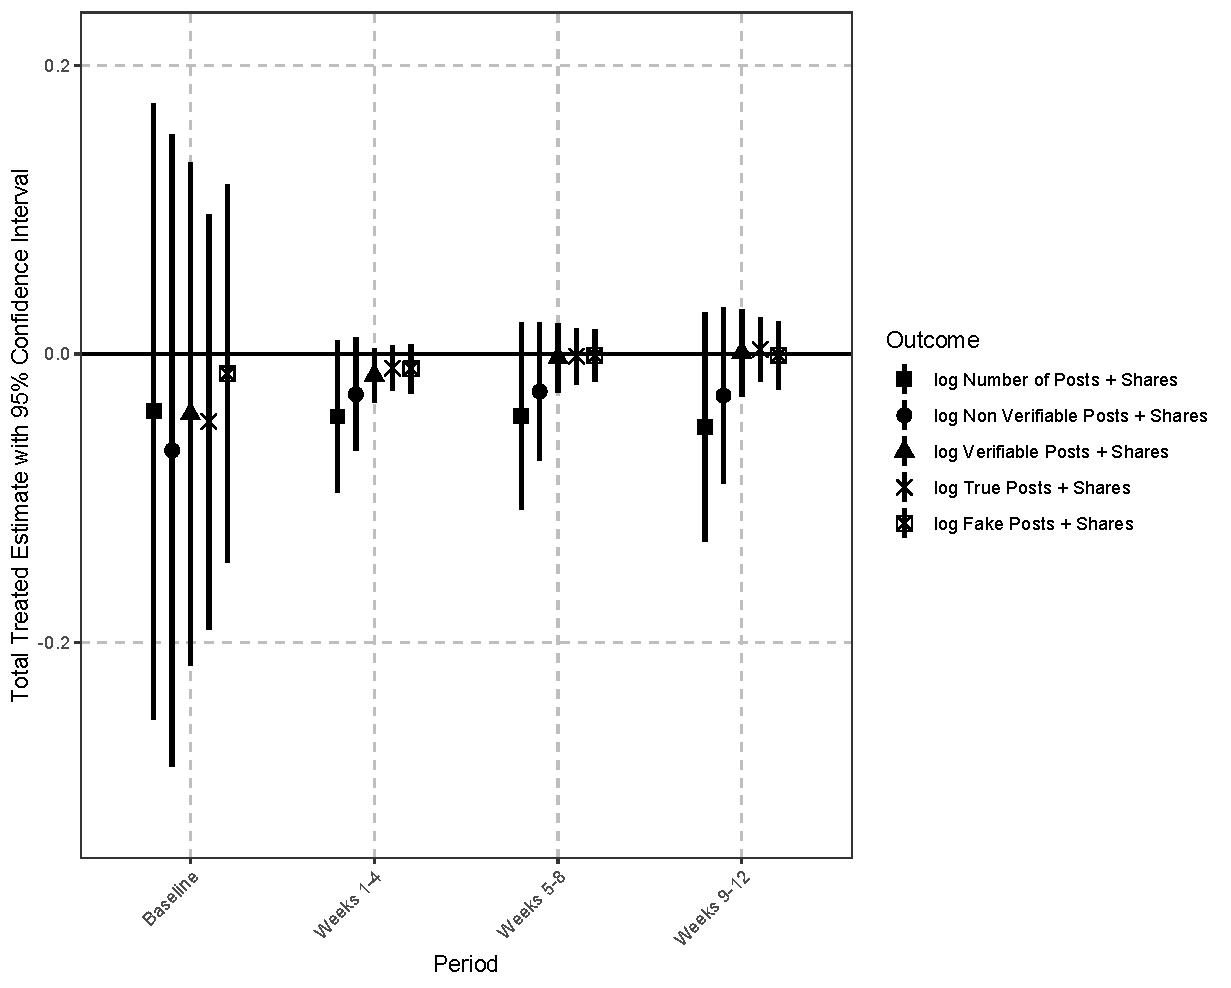
\includegraphics[width=\textwidth]{../results/replots/extensive_linear_90p_p5_with_baseline/log_extensive_verifiability_fes_normal_p90_p5_b1_500perm_with_baseline.pdf}
    \label{fig:extensive_b1_baseline_endline}
    \floatfoot{\textit{Notes:} The figure reports the estimated effect of treatment for the Batch 1 sample, combining the baseline specification with the endline specifications for Weeks 1--4, Weeks 5--8, and Weeks 9--12. Whiskers denote permutation-based 95\% confidence intervals.}
\end{figure}

\subsection{Robustness: Strong Followers Only, Batch 1}

\begin{figure}[!htbp]
    \centering
    \caption{Extensive Outcomes: Baseline and Endline Effects, Strong-Follower Sample, Batch 1}
    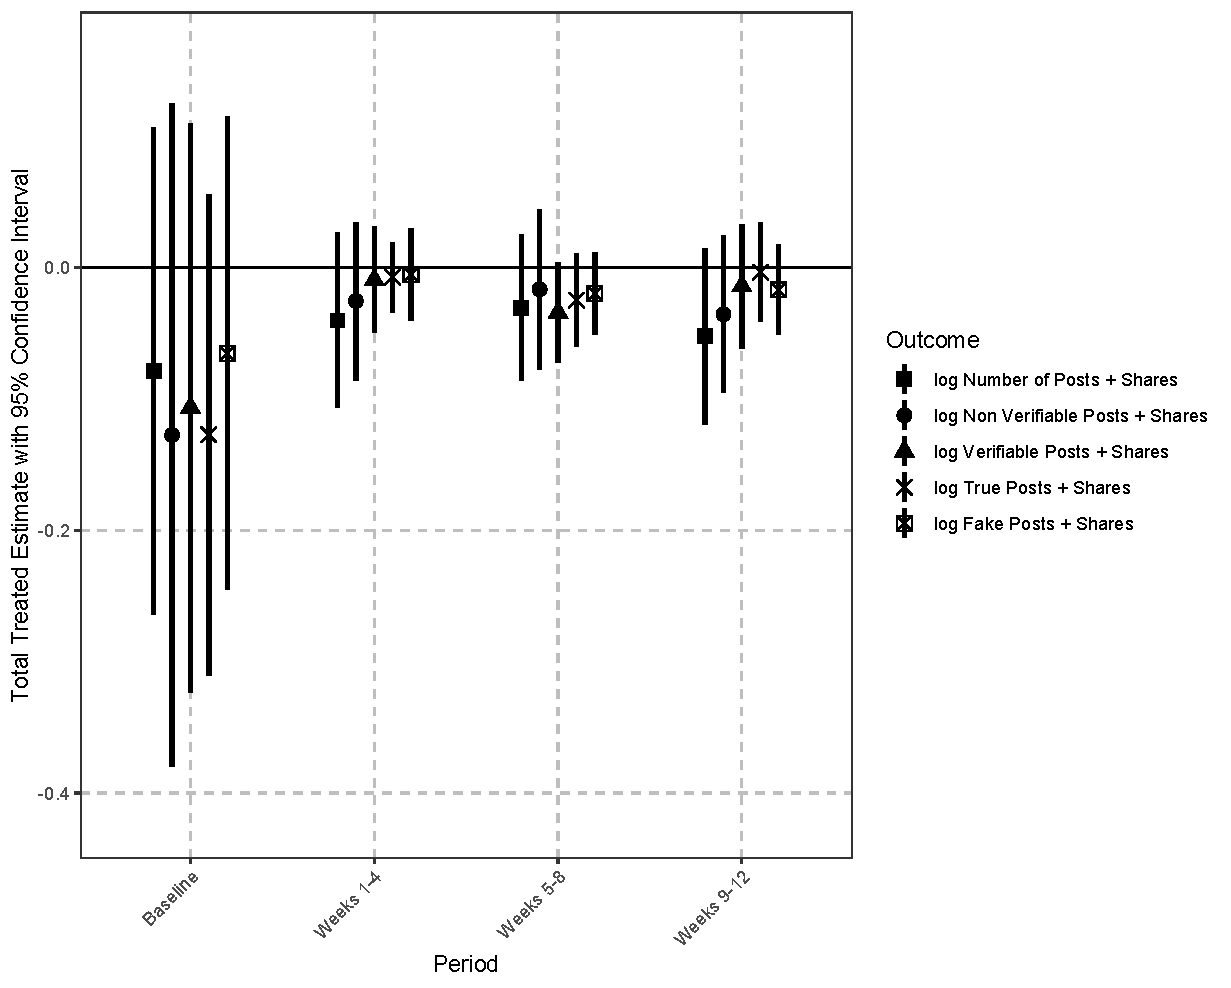
\includegraphics[width=\textwidth]{../results/replots/extensive_linear_90p_p5_strong_with_baseline/log_extensive_verifiability_fes_normal_p90_p5_strong_b1_500perm_with_baseline.pdf}
    \label{fig:extensive_strong_b1_baseline_endline}
    \floatfoot{\textit{Notes:} The figure reports the estimated effect of treatment for the Batch 1 sample restricted to followers with at least one strong treated connection. Whiskers denote permutation-based 95\% confidence intervals.}
\end{figure}


\input{v1_paper/discussion}

\input{v1_paper/conclusion}


\clearpage
\bibliographystyle{apsr}
\typeout{}

\singlespacing

\bibliographystyle{apsr}
\bibliography{mercury}

\clearpage

\appendix

\setcounter{table}{0}
\setcounter{figure}{0}
\renewcommand{\thetable}{A\arabic{table}}
\renewcommand{\thefigure}{A\arabic{figure}}

\section{Appendix Results}
\label{app:results_appendix}

\subsection{Batch 1 Stage-by-Stage Results}

\begin{figure}[!htbp]
    \centering
    \caption{Extensive Outcomes: Stage-by-Stage Effects, Batch 1}
    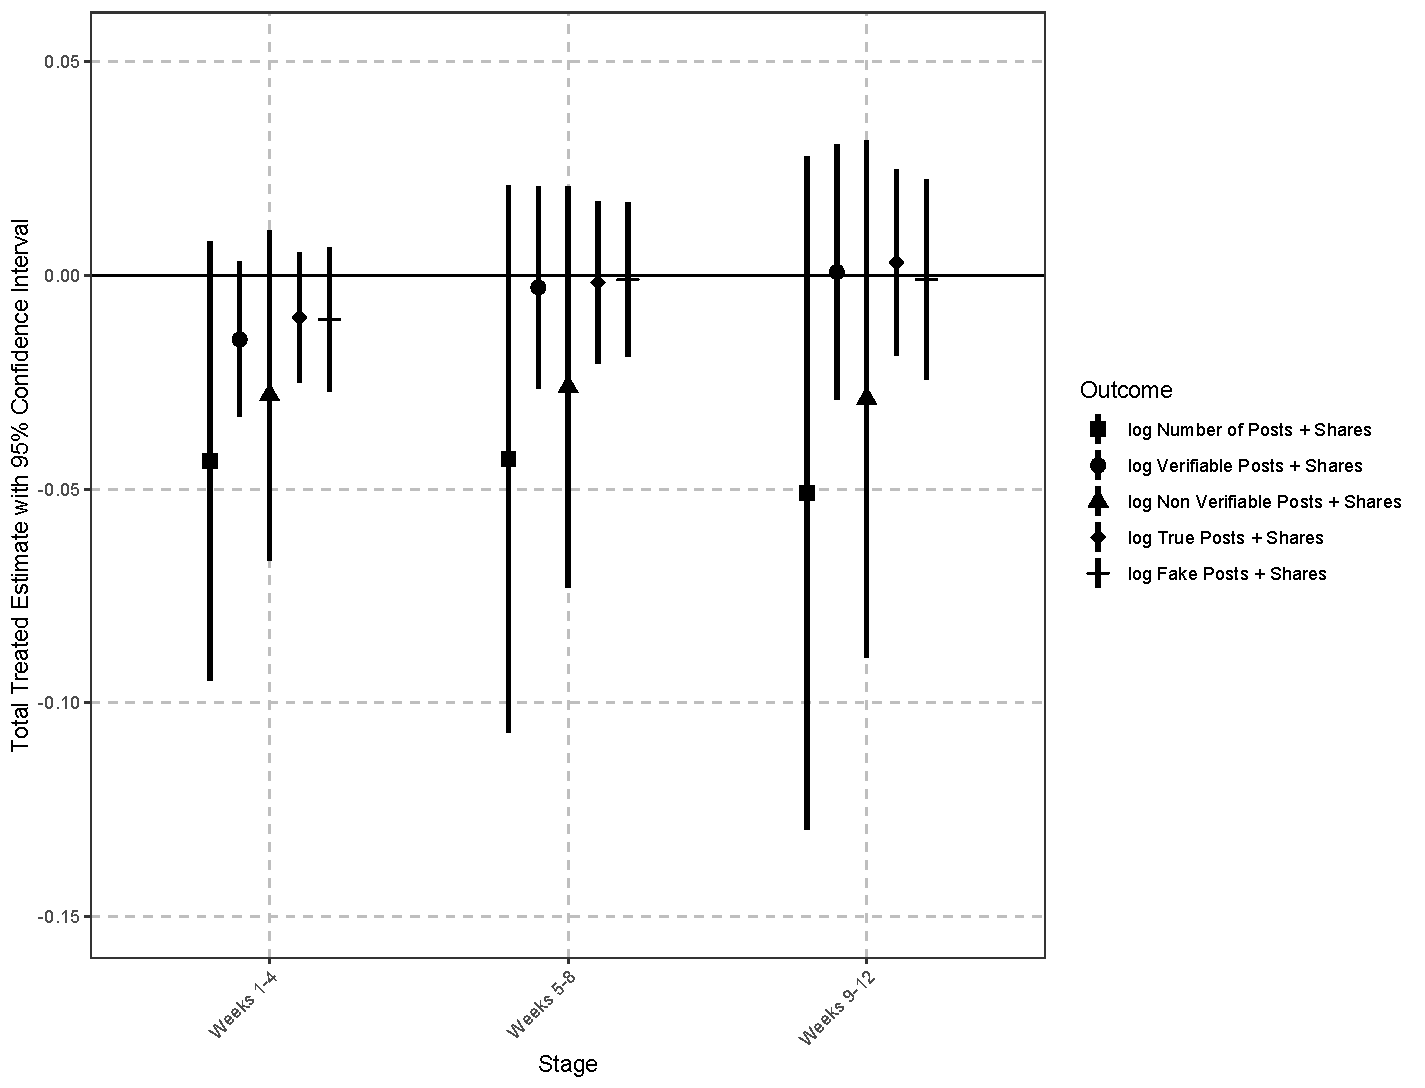
\includegraphics[width=\textwidth]{../results/replots/extensive_linear_90p_p5/log_extensive_verifiability_fes_normal_p90_p5_b1_1000perm.pdf}
    \label{fig:appendix_extensive_stage_b1}
    \floatfoot{\textit{Notes:} The figure reports the estimated effect of treatment for the Batch 1 extensive-margin sample separately for Weeks 1--4, Weeks 5--8, and Weeks 9--12. Whiskers denote permutation-based 95\% confidence intervals.}
\end{figure}

\begin{figure}[!htbp]
    \centering
    \caption{Extensive Outcomes: Stage-by-Stage Effects, Strong-Follower Sample, Batch 1}
    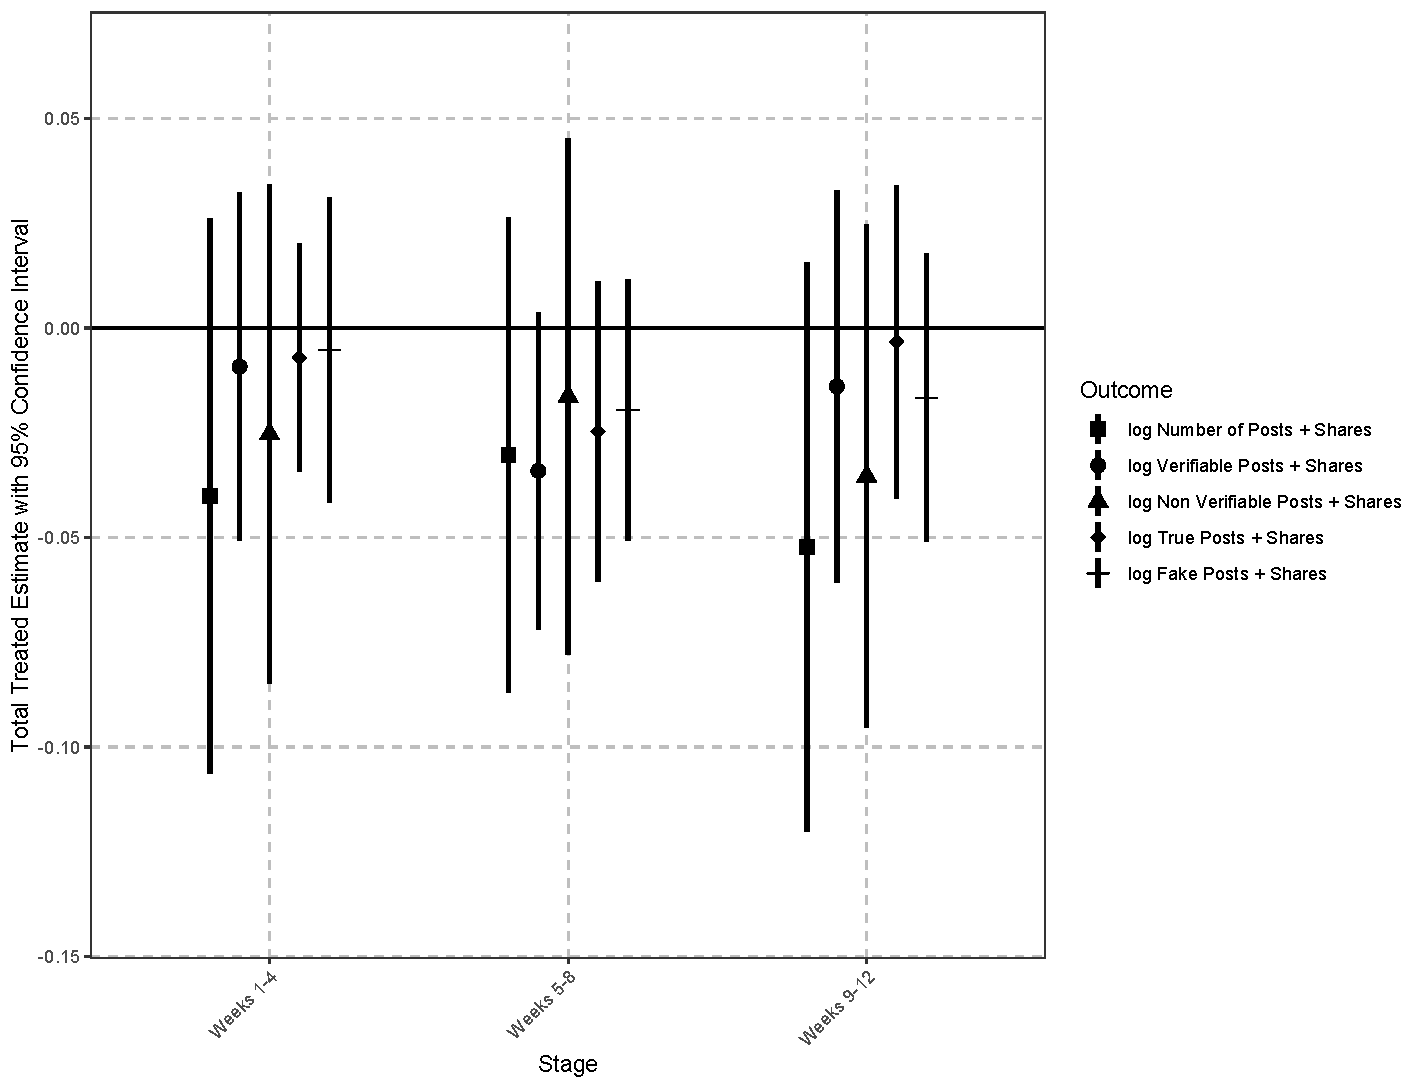
\includegraphics[width=\textwidth]{../results/replots/extensive_linear_90p_p5_strong/log_extensive_verifiability_fes_normal_p90_p5_strong_b1_1000perm.pdf}
    \label{fig:appendix_extensive_stage_strong_b1}
    \floatfoot{\textit{Notes:} The figure reports the estimated effect of treatment for the Batch 1 strong-follower sample separately for Weeks 1--4, Weeks 5--8, and Weeks 9--12. Whiskers denote permutation-based 95\% confidence intervals.}
\end{figure}

\begin{figure}[!htbp]
    \centering
    \caption{Intensive Outcomes: Stage-by-Stage Effects, Batch 1}
    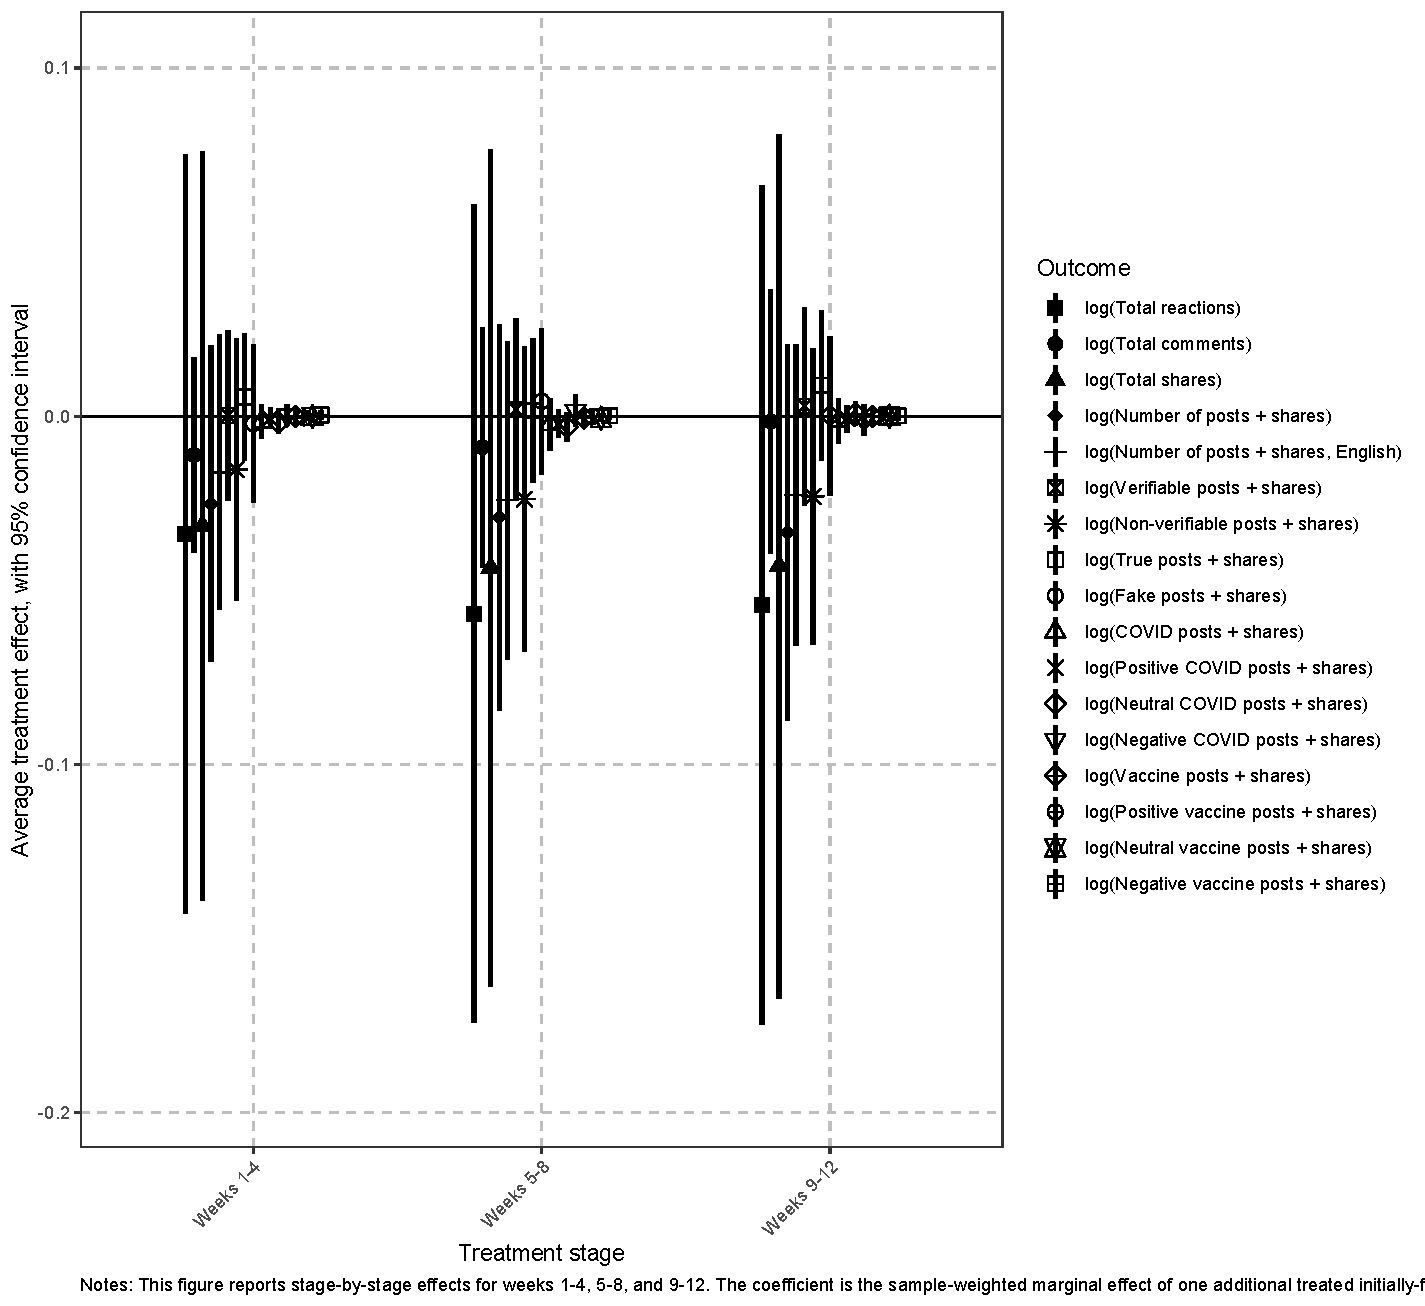
\includegraphics[width=\textwidth]{../results/replots/intensive_linear_95p_weighted/log_intensive_linear_95p_weighted_b1_1000perm.pdf}
    \label{fig:appendix_intensive_stage_b1}
    \floatfoot{\textit{Notes:} The figure reports the estimated effect of treatment for the Batch 1 intensive-margin sample separately for Weeks 1--4, Weeks 5--8, and Weeks 9--12. Whiskers denote permutation-based 95\% confidence intervals.}
\end{figure}

\subsection{Batch 1 Baseline Results}

\begin{figure}[!htbp]
    \centering
    \caption{Extensive Outcomes: Baseline Effects, Batch 1}
    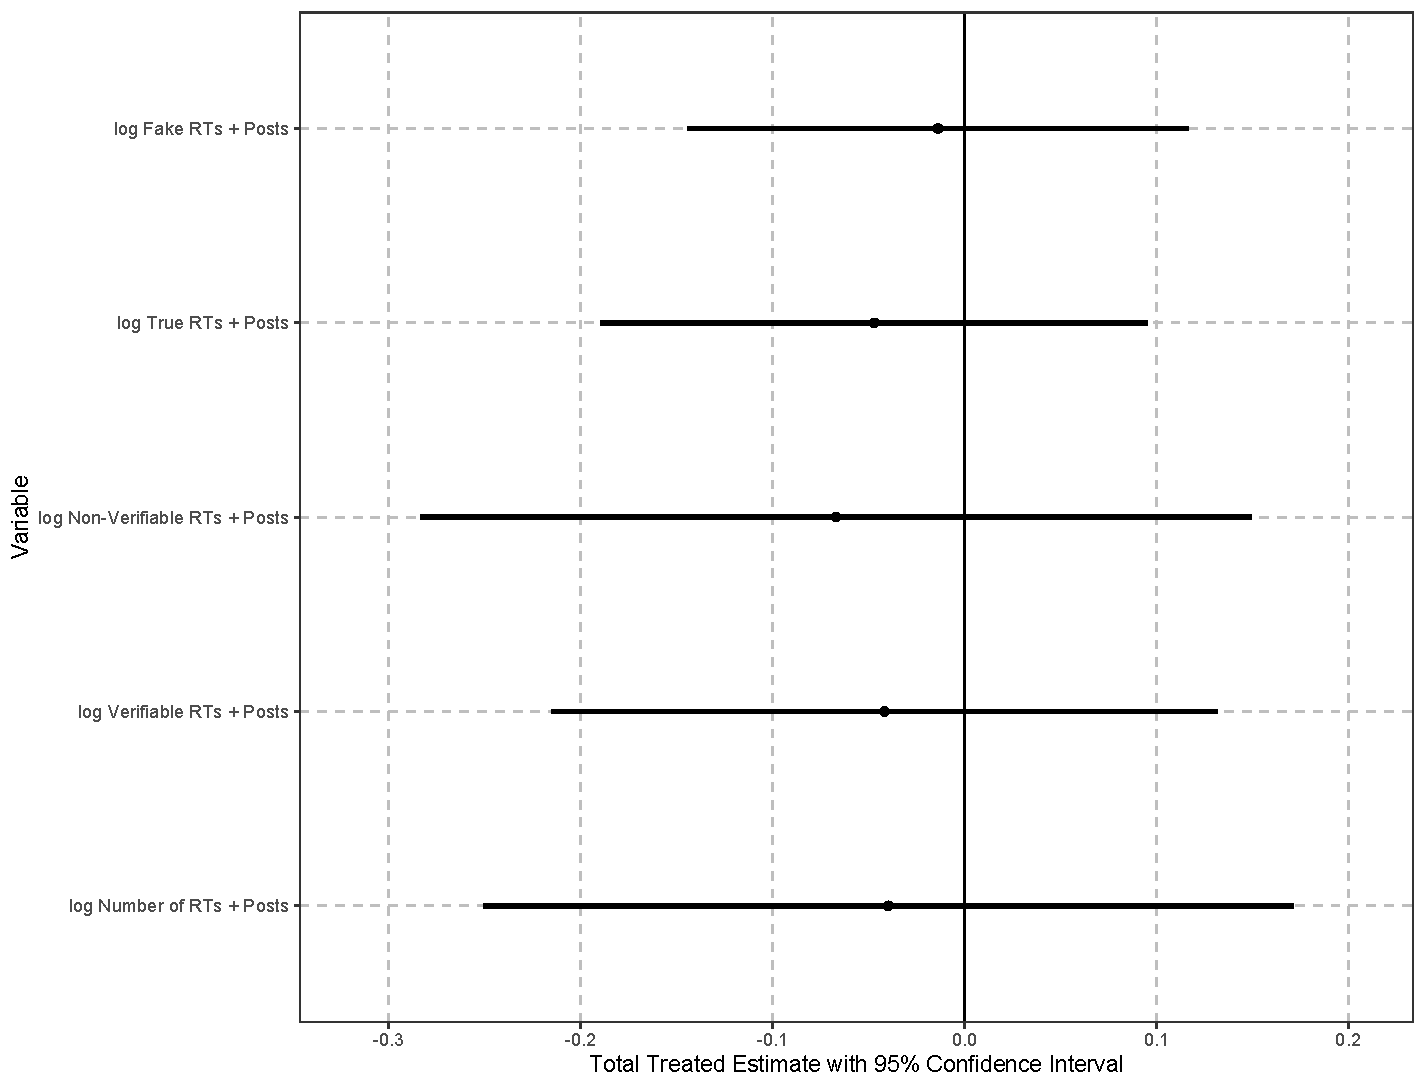
\includegraphics[width=\textwidth]{../results/replots/extensive/log_extensive_verifiability_noblockfes_p90_p0_b1_1000perm.pdf}
    \label{fig:appendix_extensive_baseline_b1}
    \floatfoot{\textit{Notes:} The figure reports the estimated treatment-control differences in baseline extensive outcomes for the Batch 1 sample. Whiskers denote permutation-based 95\% confidence intervals.}
\end{figure}

\begin{figure}[!htbp]
    \centering
    \caption{Extensive Outcomes: Baseline Effects, Strong-Follower Sample, Batch 1}
    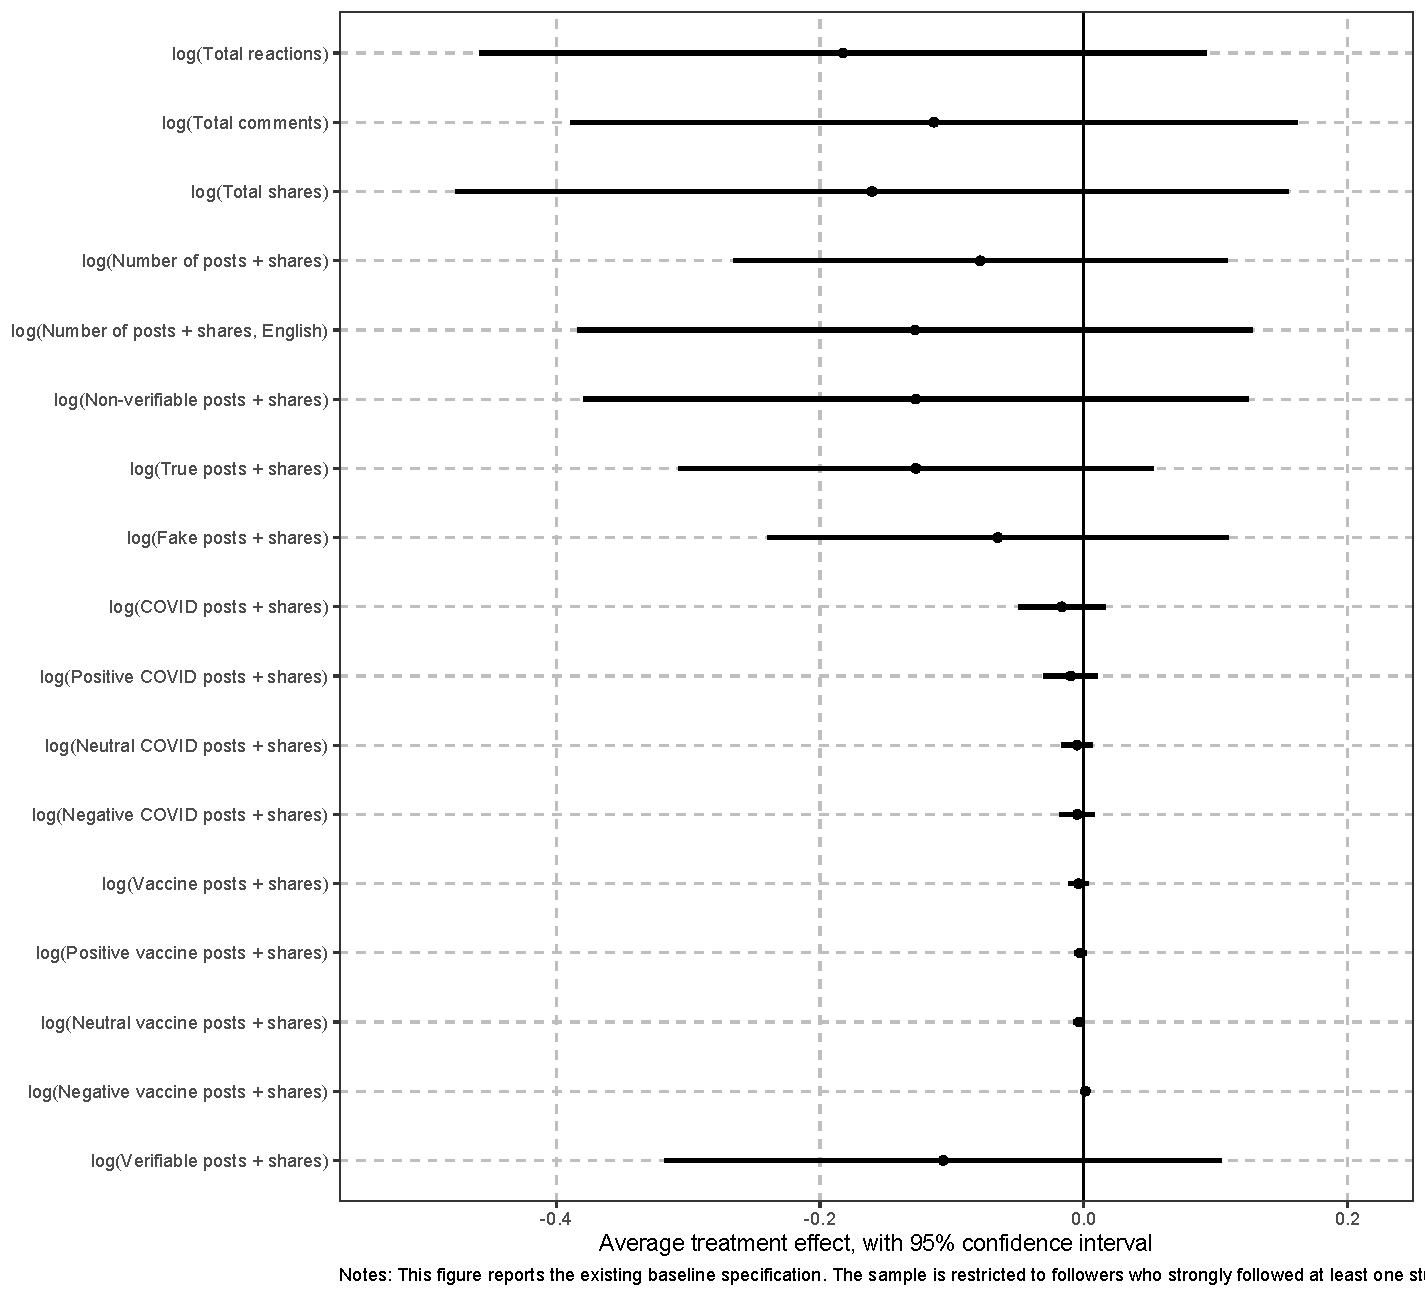
\includegraphics[width=\textwidth]{../results/replots/extensive_strong/log_extensive_verifiability_noblockfes_p90_p0_strong_b1_1000perm.pdf}
    \label{fig:appendix_extensive_baseline_strong_b1}
    \floatfoot{\textit{Notes:} The figure reports the estimated treatment-control differences in baseline extensive outcomes for the Batch 1 strong-follower sample. Whiskers denote permutation-based 95\% confidence intervals.}
\end{figure}

\begin{figure}[!htbp]
    \centering
    \caption{Intensive Outcomes: Baseline Effects, Batch 1}
    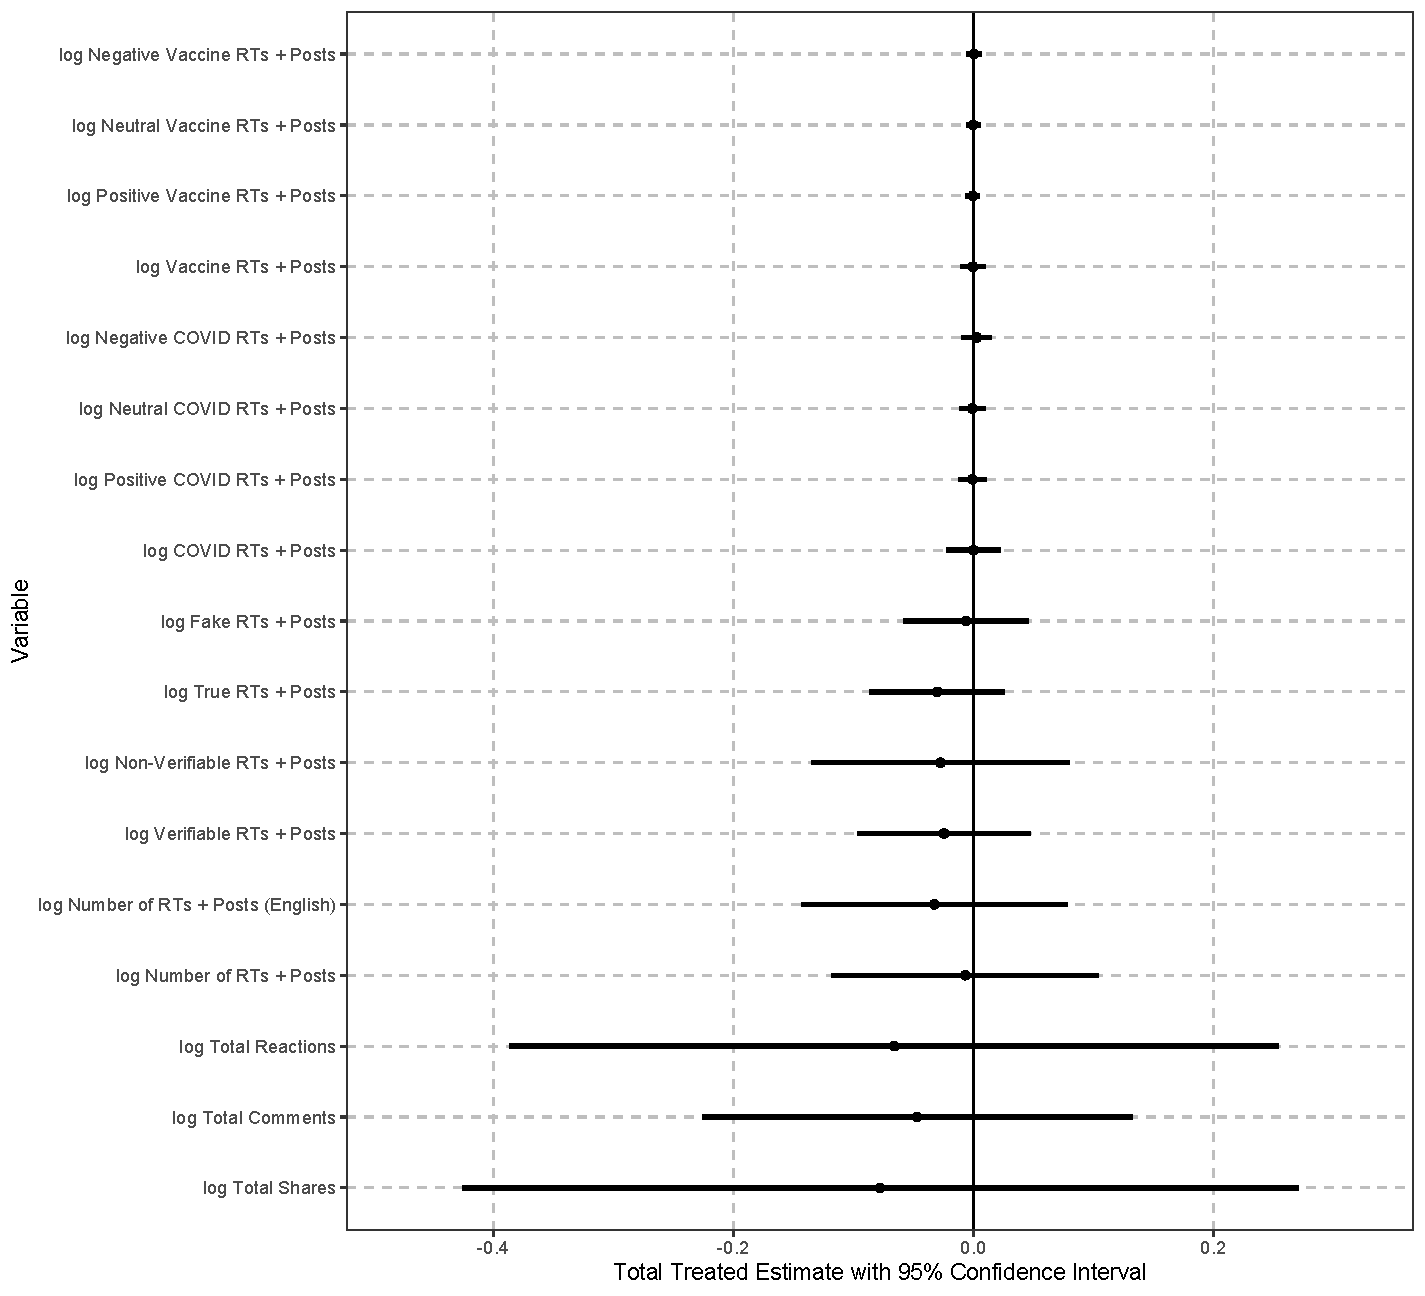
\includegraphics[width=\textwidth]{../results/replots/intensive_baseline_weighted/log_intensive_baseline_weighted_b1_1000perm.pdf}
    \label{fig:appendix_intensive_baseline_b1}
    \floatfoot{\textit{Notes:} The figure reports the estimated treatment-control differences in baseline intensive outcomes for the Batch 1 sample. Whiskers denote permutation-based 95\% confidence intervals.}
\end{figure}

\subsection{Aggregated Batch 2 and Both-Batch Results}

\begin{figure}[!htbp]
    \centering
    \caption{Extensive Outcomes: Aggregated Treatment-Period Effects, Batch 2}
    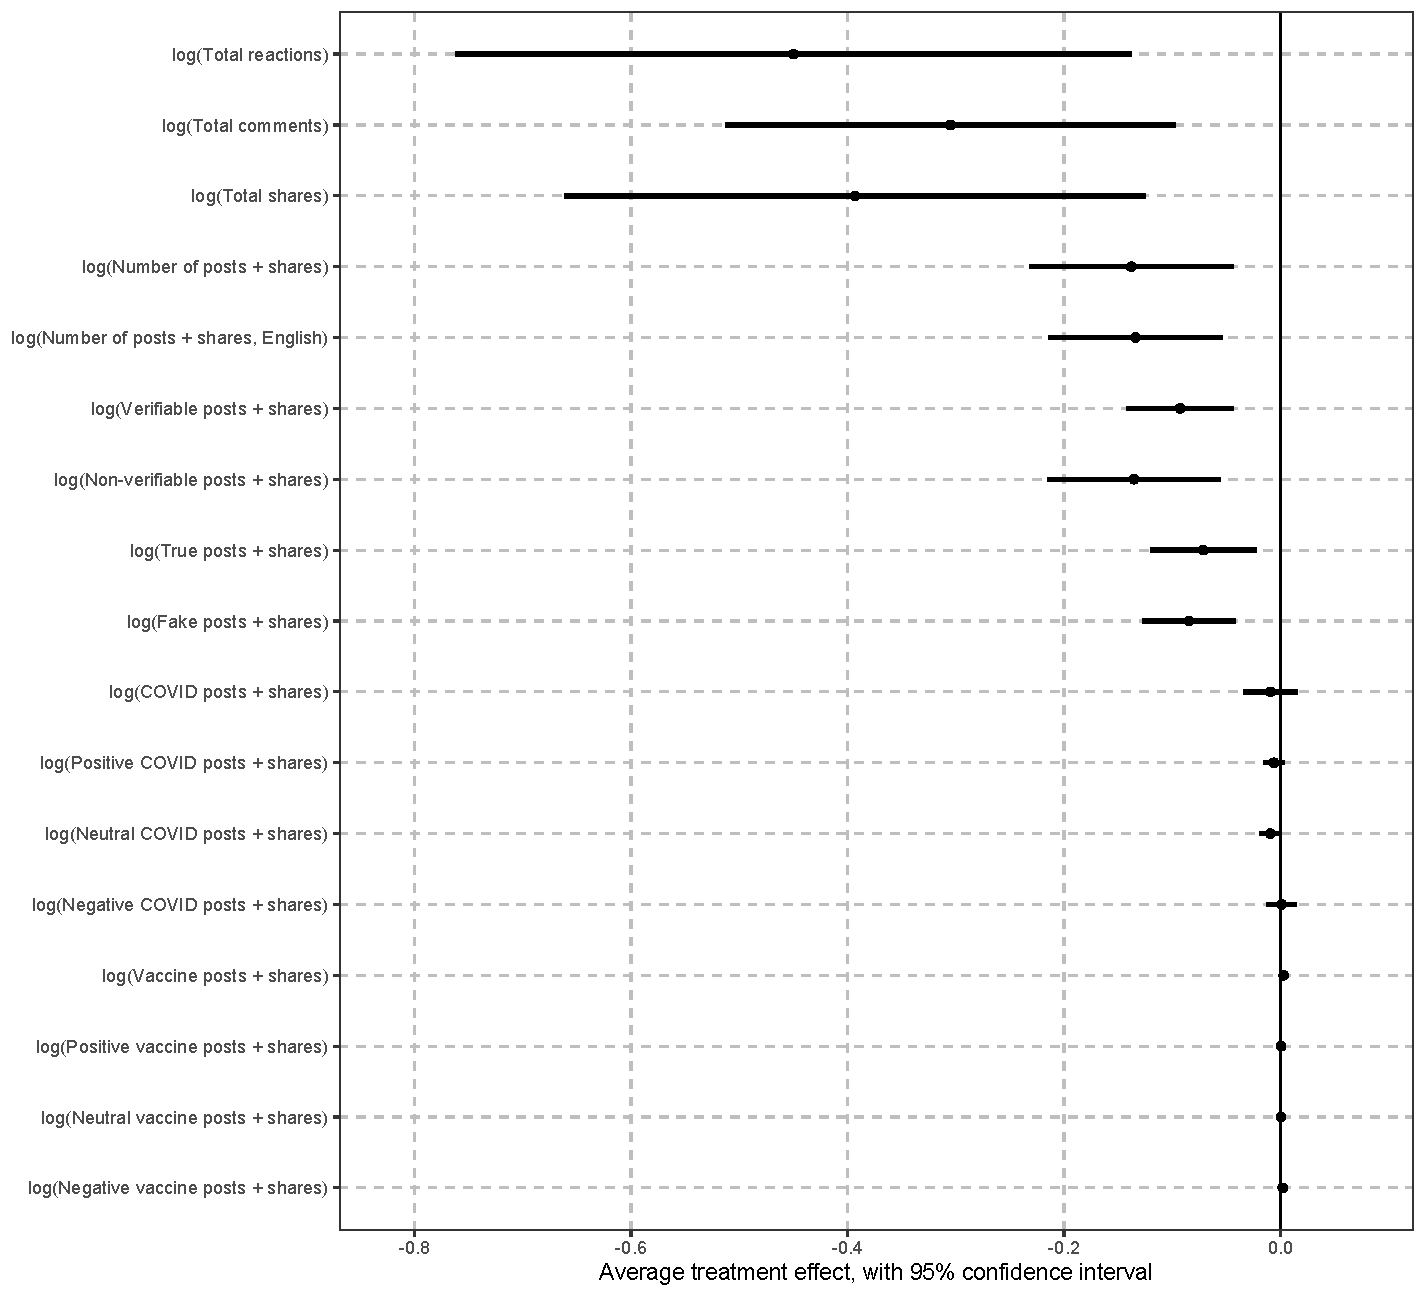
\includegraphics[width=\textwidth]{../results/replots/extensive_aggregate_batches/log_extensive_aggregate_batches_b2_1000perm.pdf}
    \label{fig:appendix_extensive_aggregate_b2}
    \floatfoot{\textit{Notes:} The figure reports the estimated effect of treatment for the Batch 2 extensive-margin sample after aggregating outcomes across Weeks 1--12. Whiskers denote permutation-based 95\% confidence intervals.}
\end{figure}

\begin{figure}[!htbp]
    \centering
    \caption{Extensive Outcomes: Aggregated Treatment-Period Effects, Both Batches}
    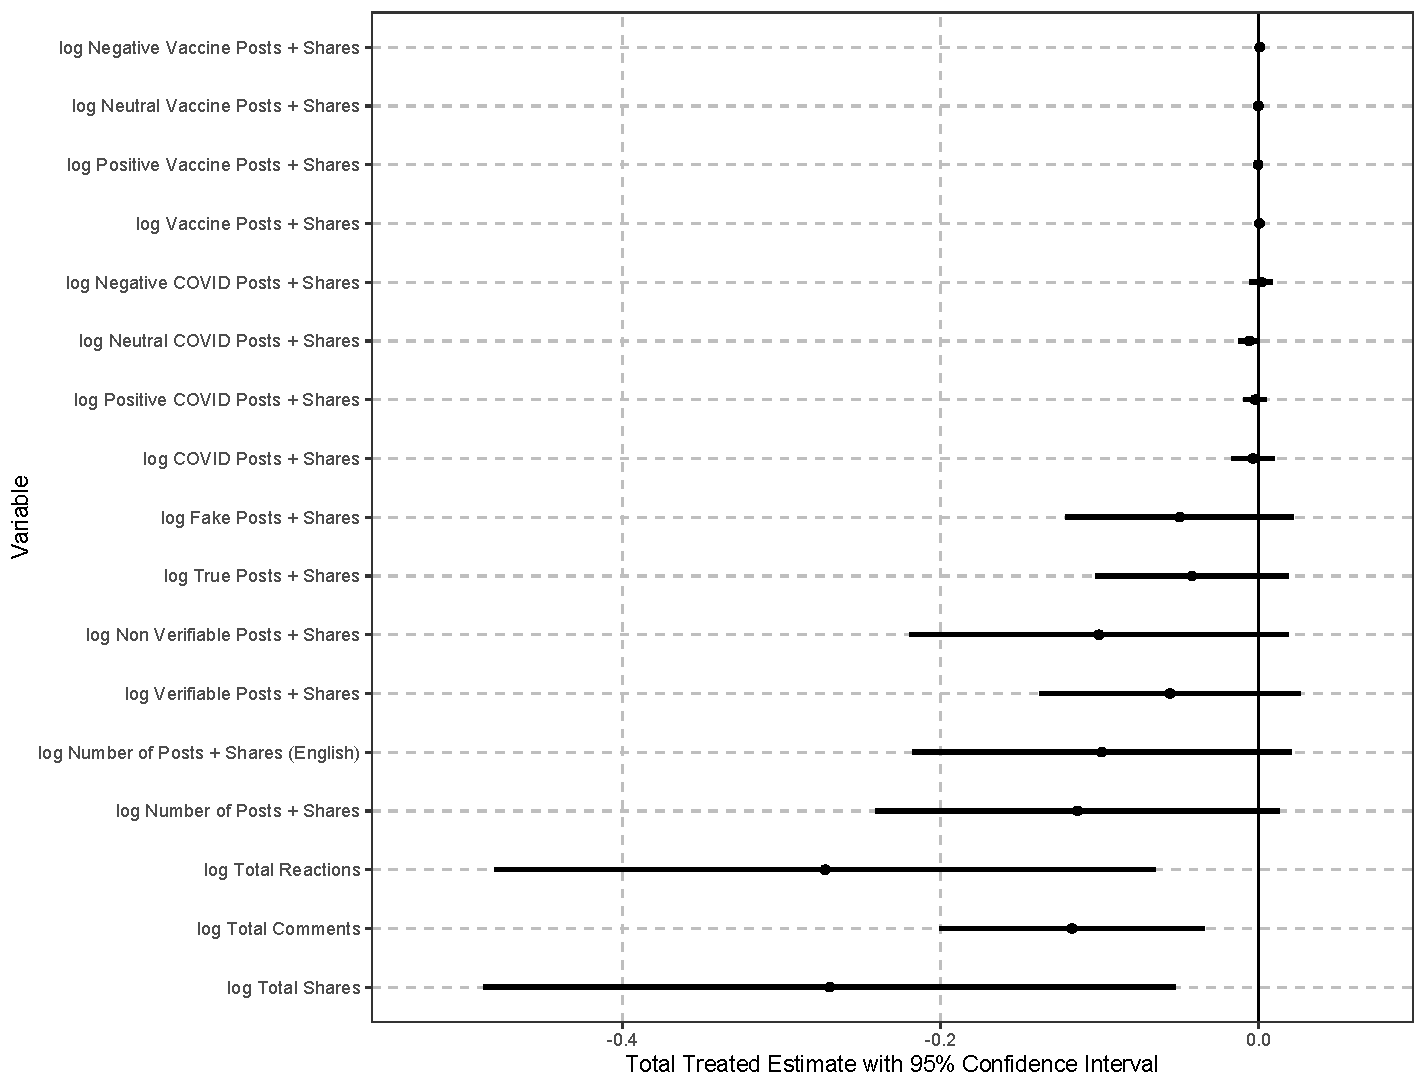
\includegraphics[width=\textwidth]{../results/replots/extensive_aggregate_batches/log_extensive_aggregate_batches_both_1000perm.pdf}
    \label{fig:appendix_extensive_aggregate_both}
    \floatfoot{\textit{Notes:} The figure reports the estimated effect of treatment for the pooled extensive-margin sample after aggregating outcomes across Weeks 1--12. Whiskers denote permutation-based 95\% confidence intervals.}
\end{figure}

\begin{figure}[!htbp]
    \centering
    \caption{Intensive Outcomes: Aggregated Treatment-Period Effects, Batch 2}
    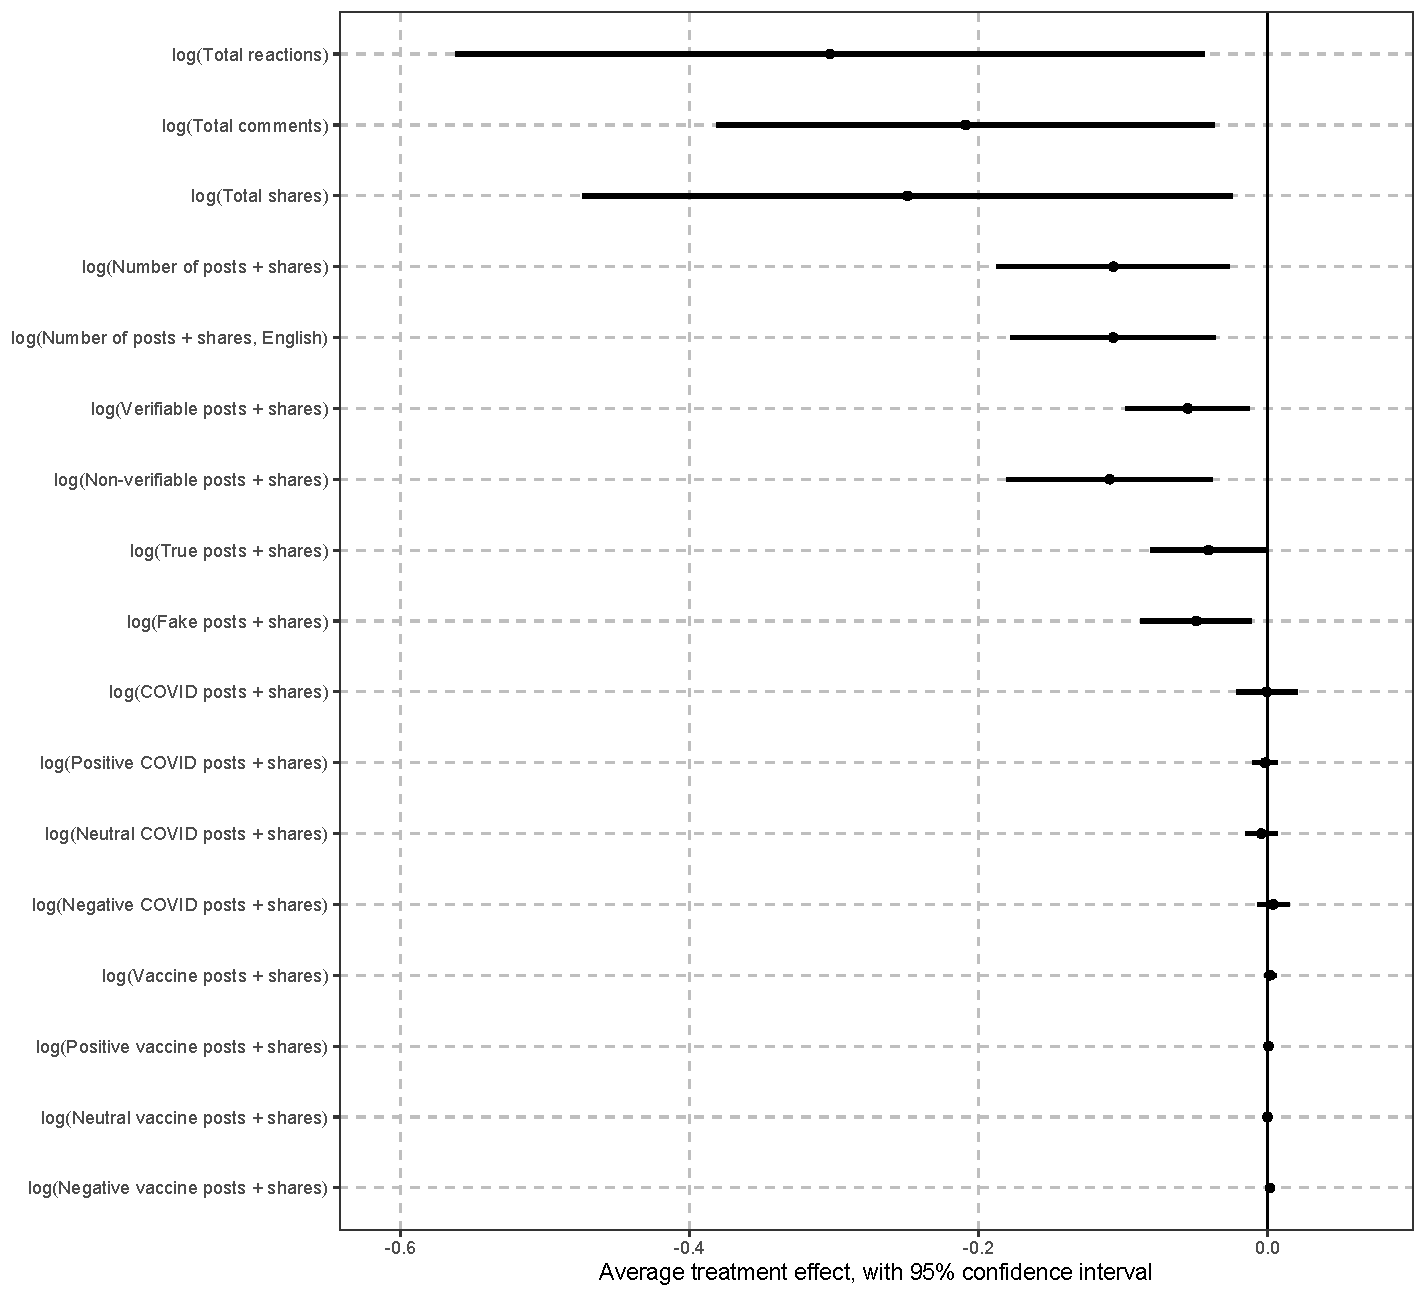
\includegraphics[width=\textwidth]{../results/replots/intensive_aggregate_batches/log_intensive_aggregate_batches_b2_1000perm.pdf}
    \label{fig:appendix_intensive_aggregate_b2}
    \floatfoot{\textit{Notes:} The figure reports the estimated effect of treatment for the Batch 2 intensive-margin sample after aggregating outcomes across Weeks 1--12. Whiskers denote permutation-based 95\% confidence intervals.}
\end{figure}

\begin{figure}[!htbp]
    \centering
    \caption{Intensive Outcomes: Aggregated Treatment-Period Effects, Both Batches}
    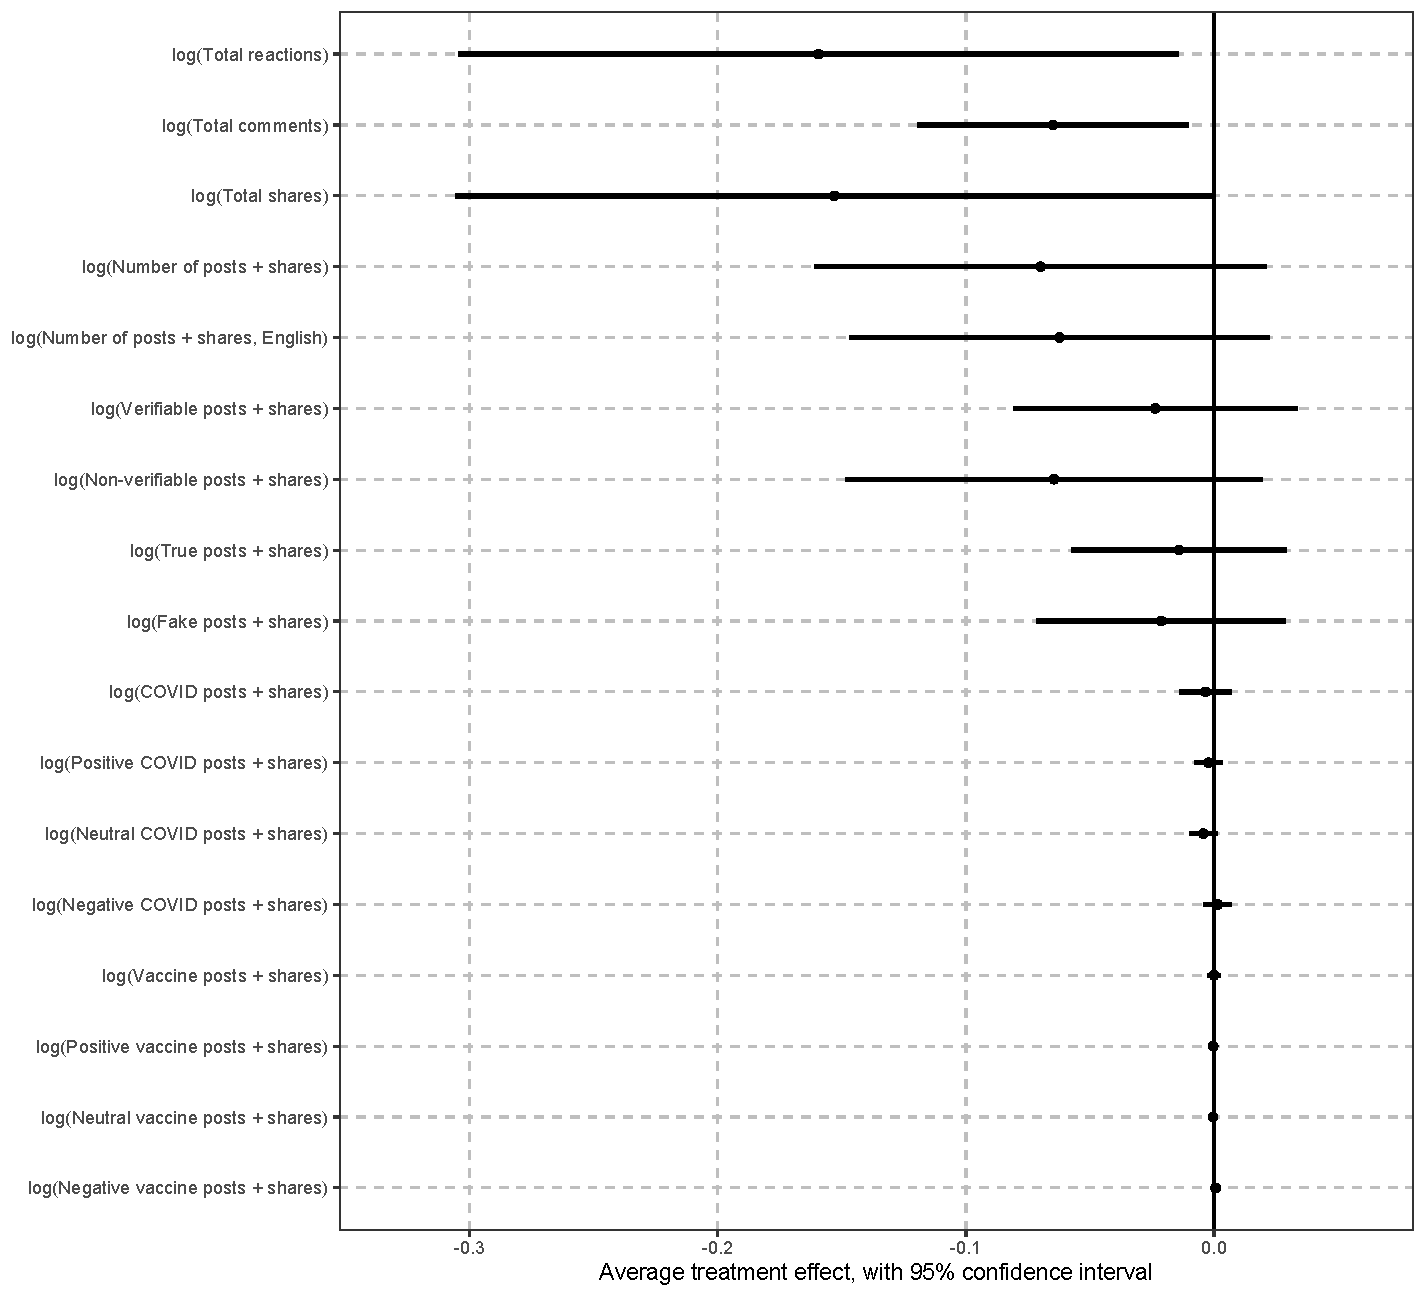
\includegraphics[width=\textwidth]{../results/replots/intensive_aggregate_batches/log_intensive_aggregate_batches_both_1000perm.pdf}
    \label{fig:appendix_intensive_aggregate_both}
    \floatfoot{\textit{Notes:} The figure reports the estimated effect of treatment for the pooled intensive-margin sample after aggregating outcomes across Weeks 1--12. Whiskers denote permutation-based 95\% confidence intervals.}
\end{figure}

\subsection{Remaining Stage-by-Stage Results}

\begin{figure}[!htbp]
    \centering
    \caption{Extensive Outcomes: Stage-by-Stage Effects, Batch 2}
    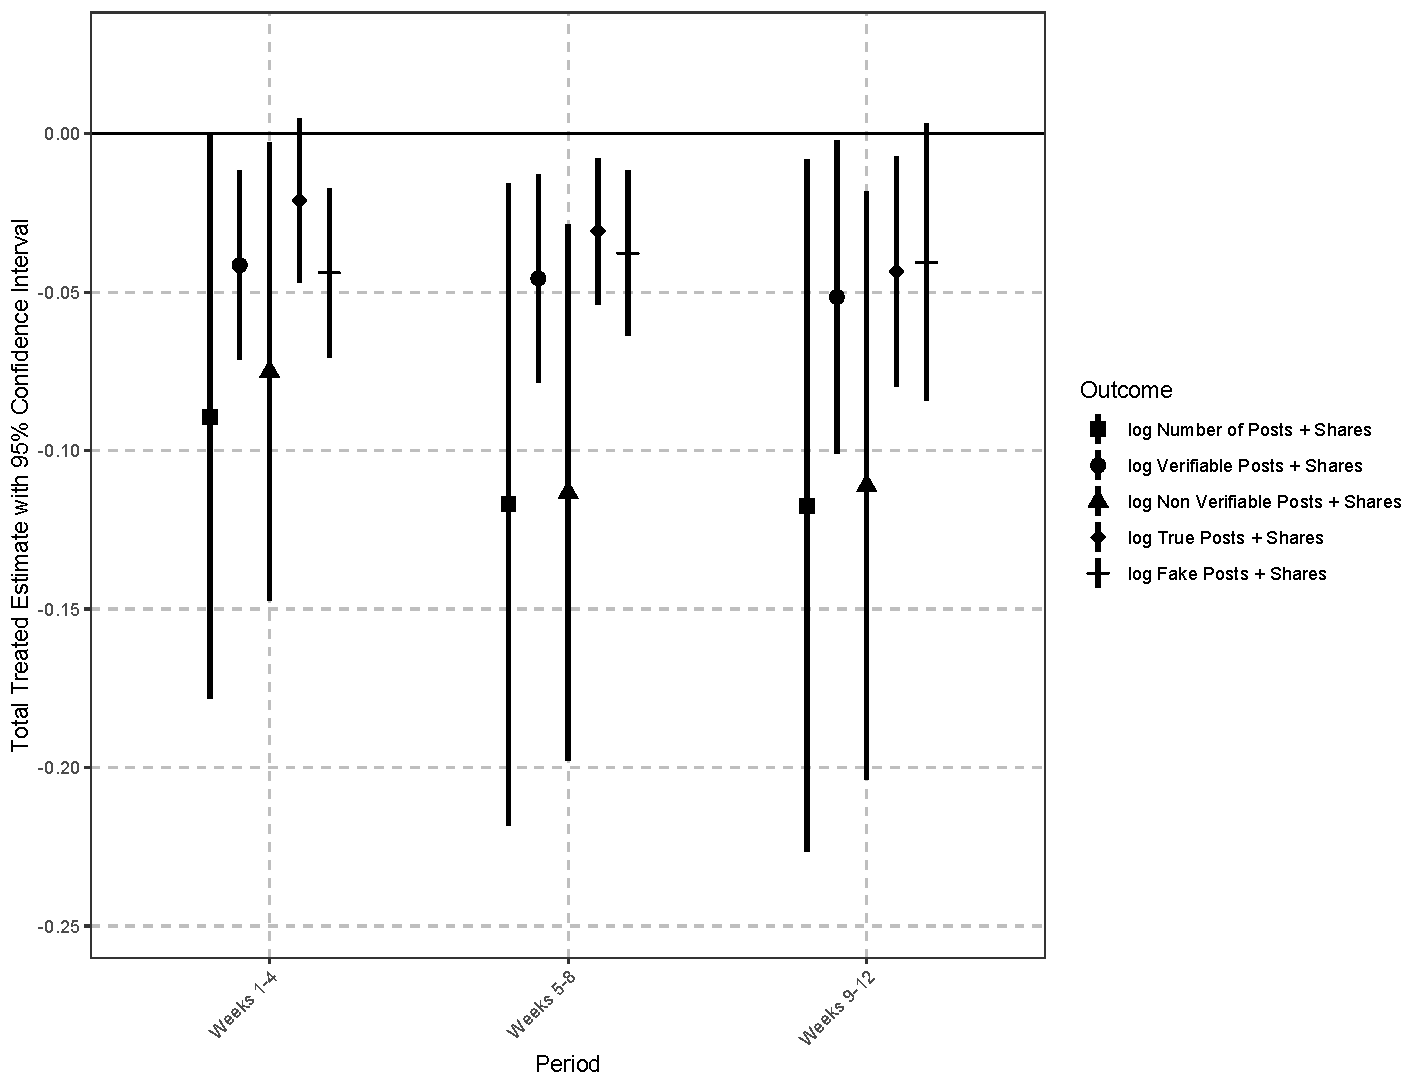
\includegraphics[width=\textwidth]{../results/replots/extensive_linear_90p_p5/log_extensive_verifiability_fes_normal_p90_p5_b2_1000perm.pdf}
    \label{fig:appendix_extensive_stage_b2}
    \floatfoot{\textit{Notes:} The figure reports the estimated effect of treatment for the Batch 2 extensive-margin sample separately for Weeks 1--4, Weeks 5--8, and Weeks 9--12. Whiskers denote permutation-based 95\% confidence intervals.}
\end{figure}

\begin{figure}[!htbp]
    \centering
    \caption{Extensive Outcomes: Stage-by-Stage Effects, Strong-Follower Sample, Batch 2}
    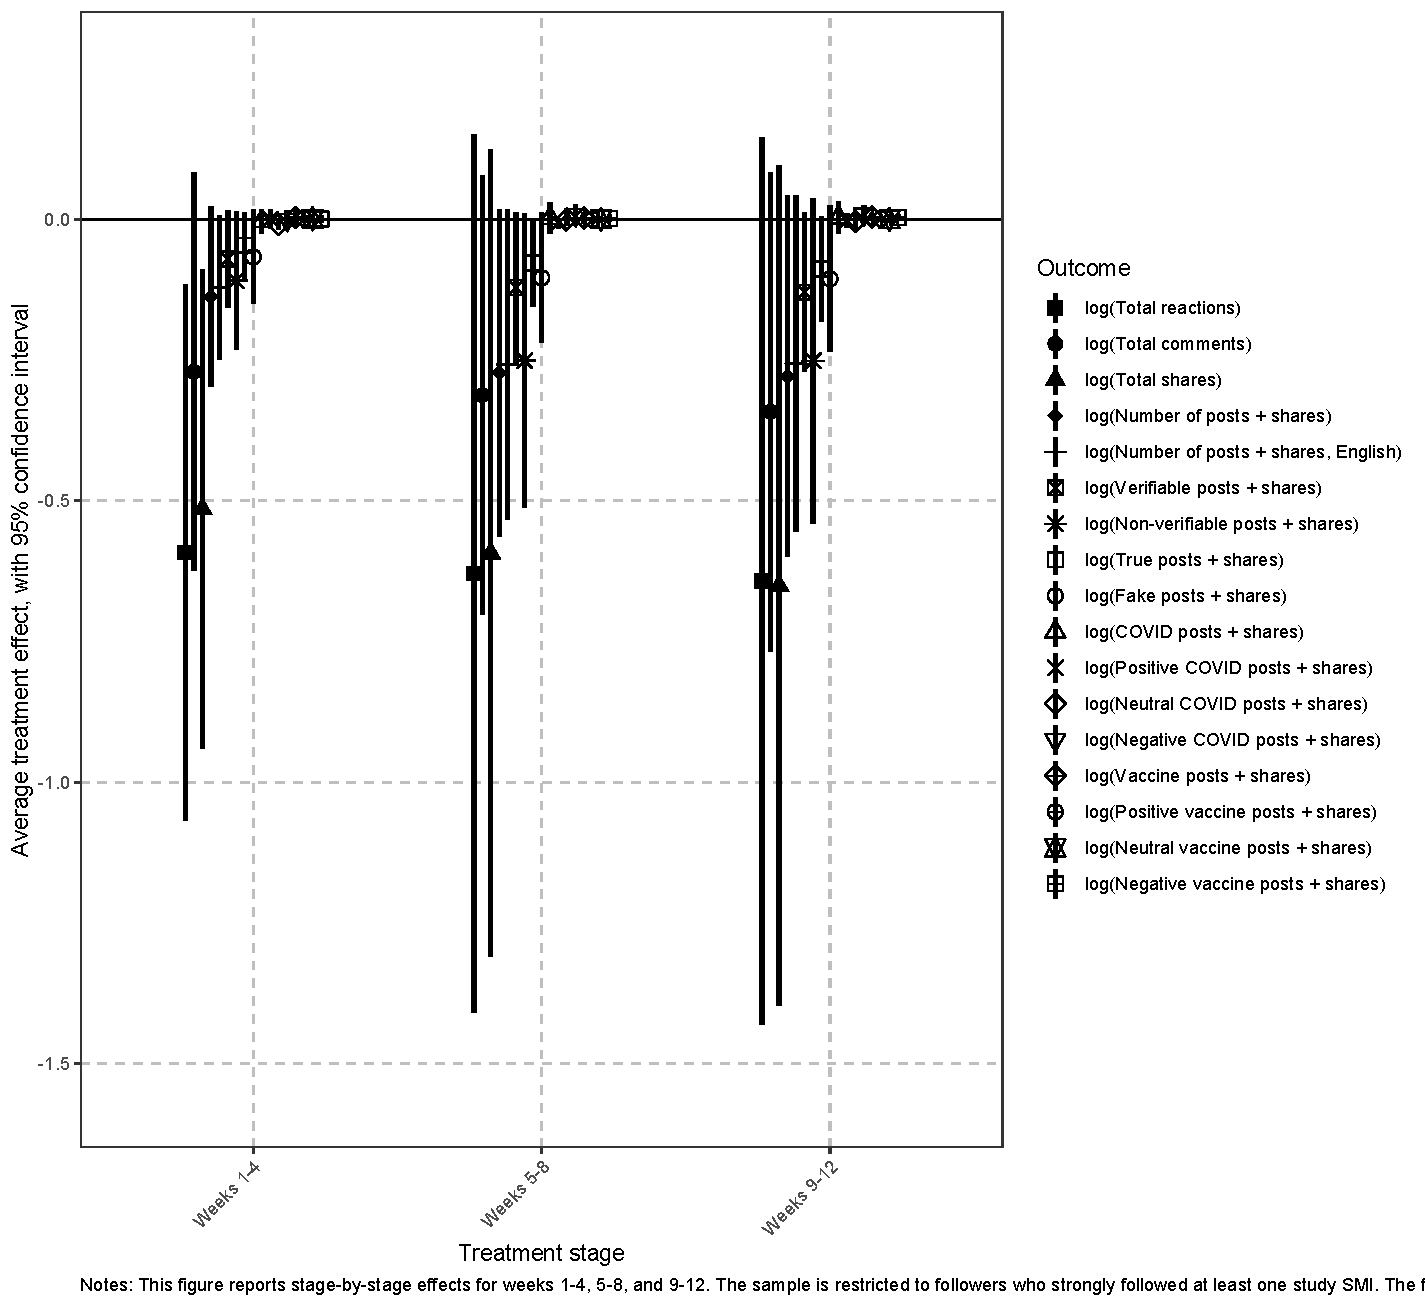
\includegraphics[width=\textwidth]{../results/replots/extensive_linear_90p_p5_strong/log_extensive_verifiability_fes_normal_p90_p5_strong_b2_1000perm.pdf}
    \label{fig:appendix_extensive_stage_strong_b2}
    \floatfoot{\textit{Notes:} The figure reports the estimated effect of treatment for the Batch 2 strong-follower sample separately for Weeks 1--4, Weeks 5--8, and Weeks 9--12. Whiskers denote permutation-based 95\% confidence intervals.}
\end{figure}

\begin{figure}[!htbp]
    \centering
    \caption{Intensive Outcomes: Stage-by-Stage Effects, Batch 2}
    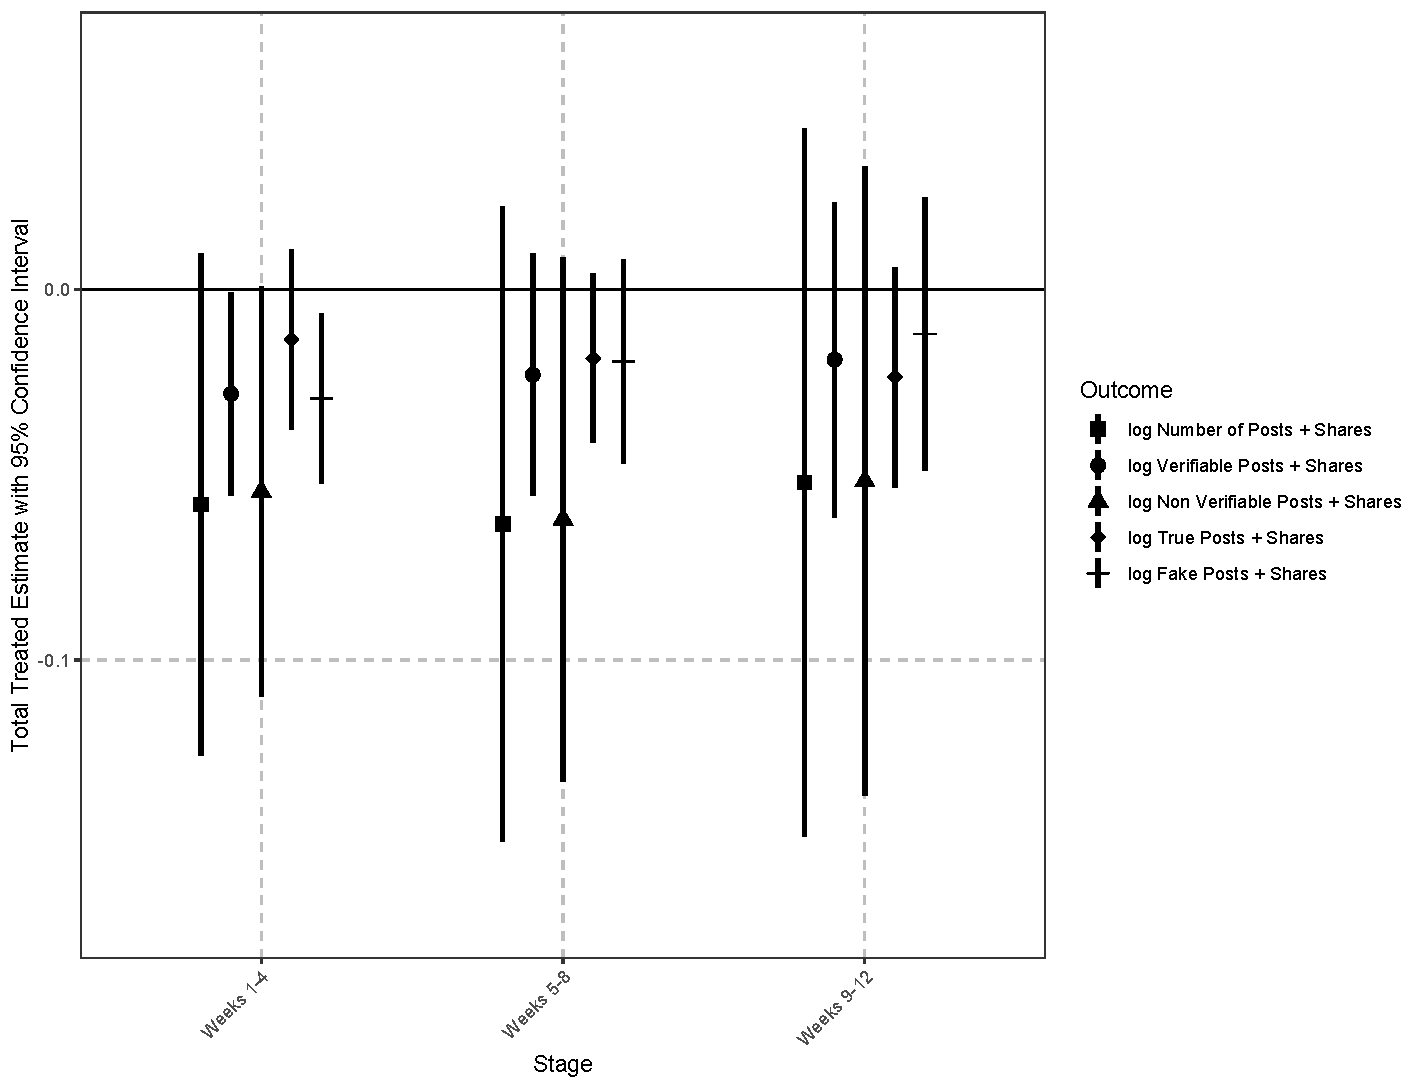
\includegraphics[width=\textwidth]{../results/replots/intensive_linear_95p_weighted/log_intensive_linear_95p_weighted_b2_1000perm.pdf}
    \label{fig:appendix_intensive_stage_b2}
    \floatfoot{\textit{Notes:} The figure reports the estimated effect of treatment for the Batch 2 intensive-margin sample separately for Weeks 1--4, Weeks 5--8, and Weeks 9--12. Whiskers denote permutation-based 95\% confidence intervals.}
\end{figure}

\begin{figure}[!htbp]
    \centering
    \caption{Extensive Outcomes: Stage-by-Stage Effects, Both Batches}
    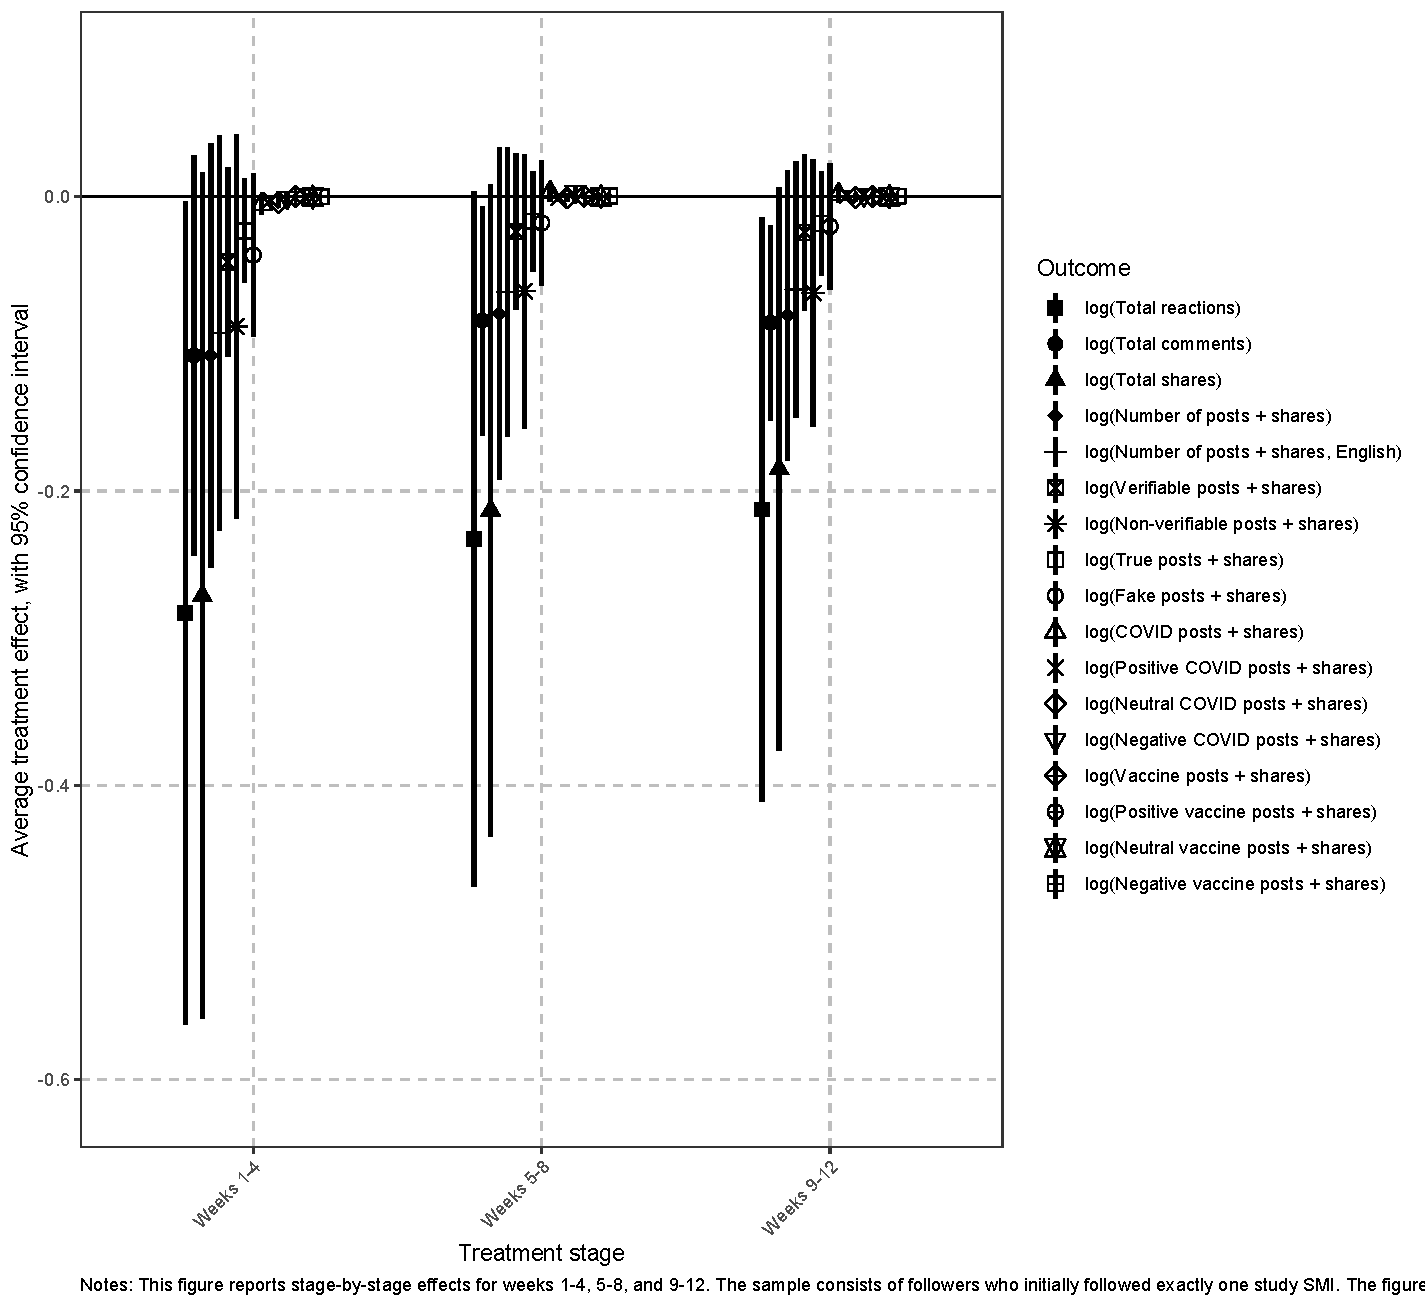
\includegraphics[width=\textwidth]{../results/replots/extensive_linear_90p_p5/log_extensive_verifiability_fes_normal_p90_p5_both_1000perm.pdf}
    \label{fig:appendix_extensive_stage_both}
    \floatfoot{\textit{Notes:} The figure reports the estimated effect of treatment for the pooled extensive-margin sample separately for Weeks 1--4, Weeks 5--8, and Weeks 9--12. Whiskers denote permutation-based 95\% confidence intervals.}
\end{figure}

\begin{figure}[!htbp]
    \centering
    \caption{Extensive Outcomes: Stage-by-Stage Effects, Strong-Follower Sample, Both Batches}
    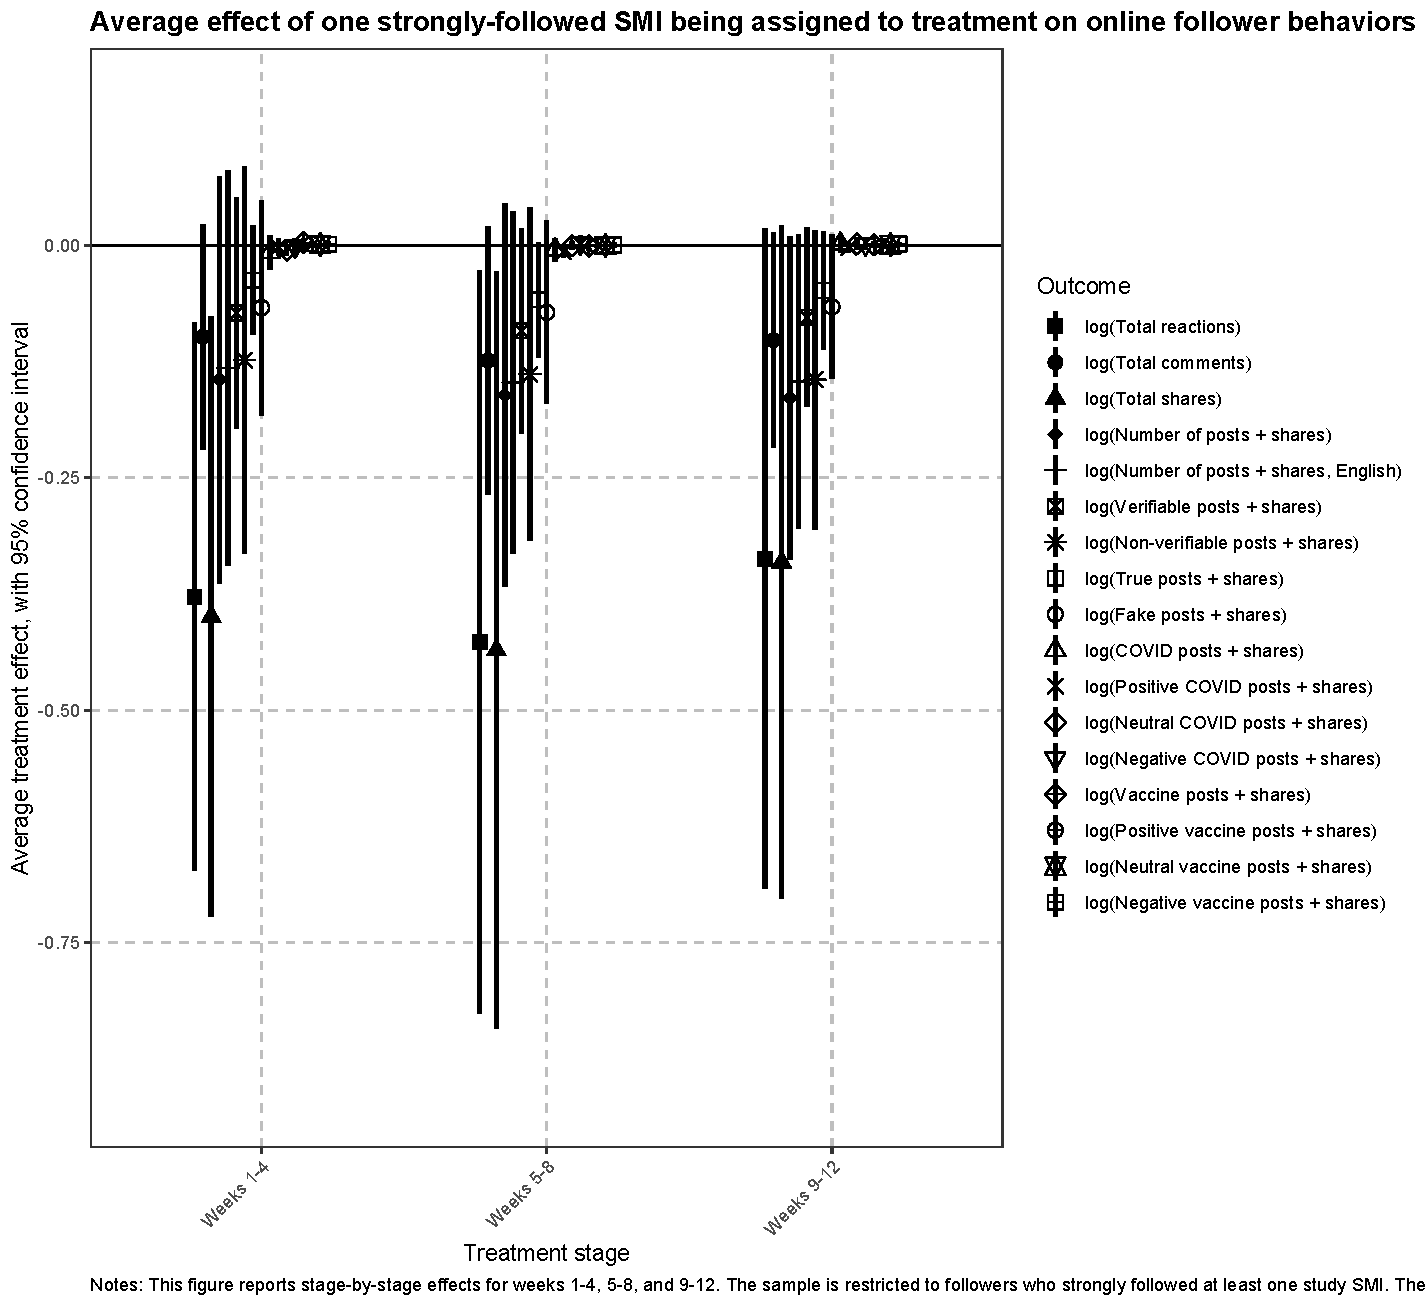
\includegraphics[width=\textwidth]{../results/replots/extensive_linear_90p_p5_strong/log_extensive_verifiability_fes_normal_p90_p5_strong_both_1000perm.pdf}
    \label{fig:appendix_extensive_stage_strong_both}
    \floatfoot{\textit{Notes:} The figure reports the estimated effect of treatment for the pooled strong-follower sample separately for Weeks 1--4, Weeks 5--8, and Weeks 9--12. Whiskers denote permutation-based 95\% confidence intervals.}
\end{figure}

\begin{figure}[!htbp]
    \centering
    \caption{Intensive Outcomes: Stage-by-Stage Effects, Both Batches}
    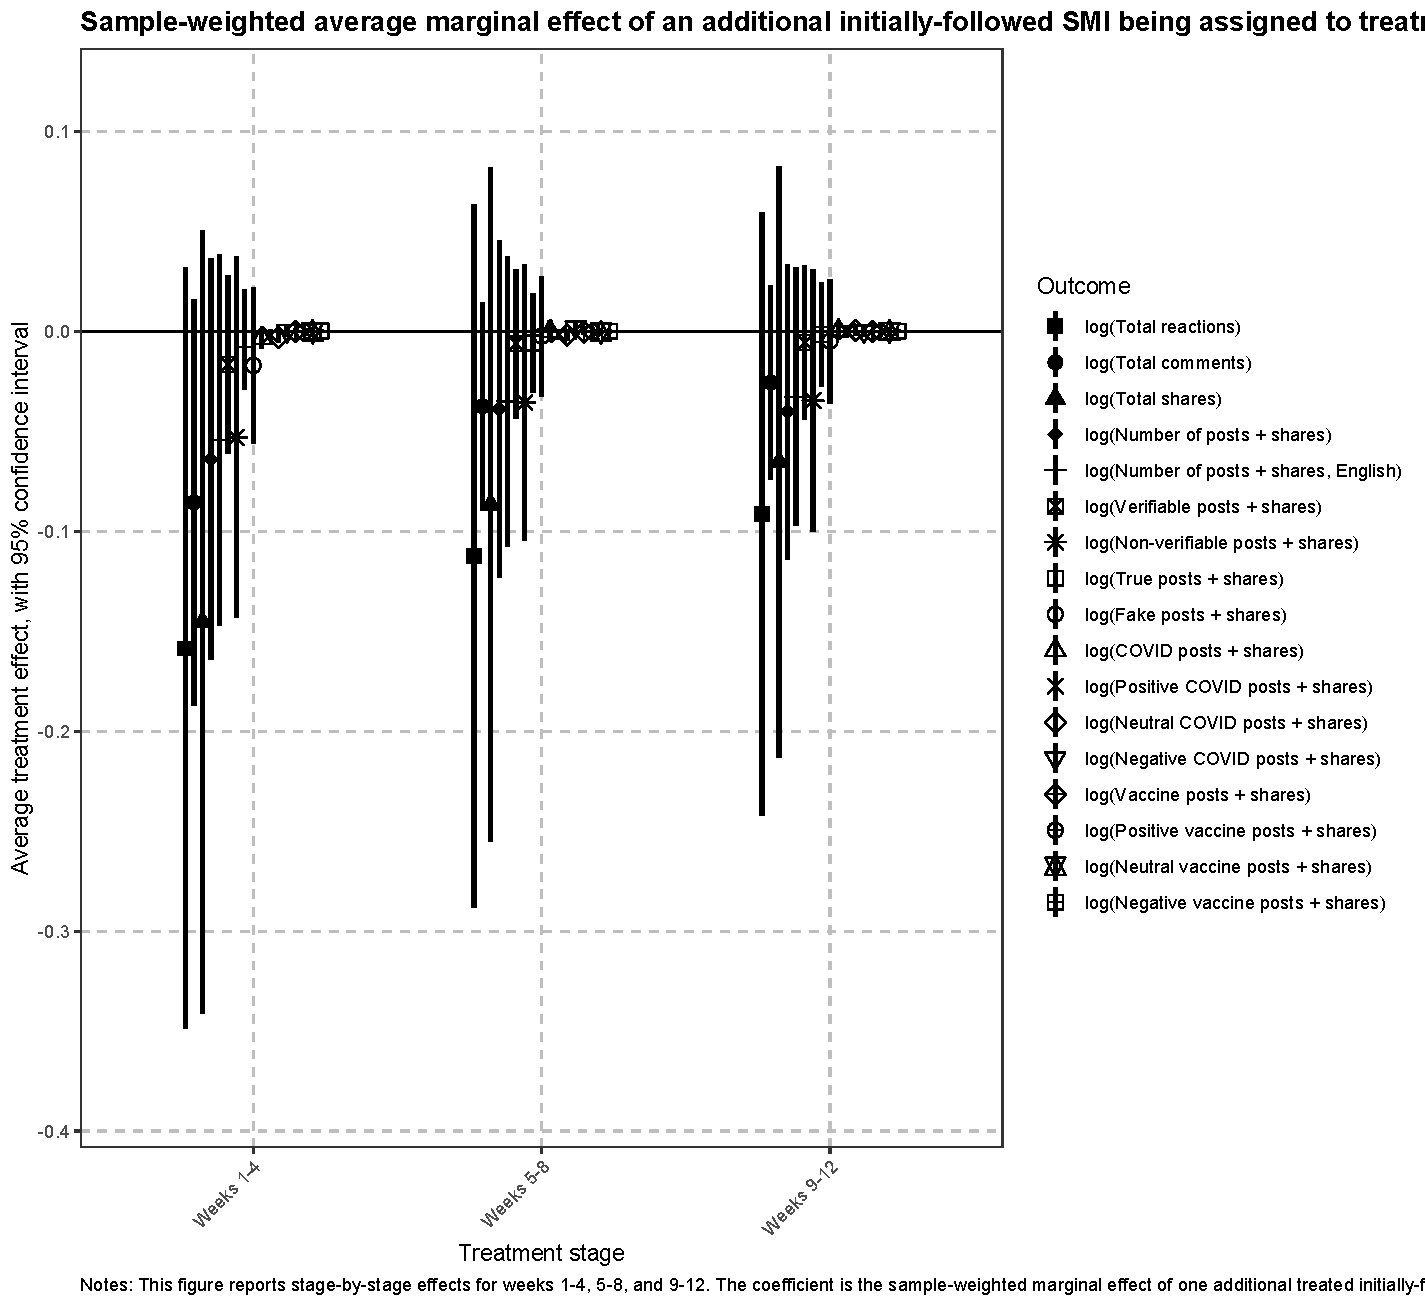
\includegraphics[width=\textwidth]{../results/replots/intensive_linear_95p_weighted/log_intensive_linear_95p_weighted_both_1000perm.pdf}
    \label{fig:appendix_intensive_stage_both}
    \floatfoot{\textit{Notes:} The figure reports the estimated effect of treatment for the pooled intensive-margin sample separately for Weeks 1--4, Weeks 5--8, and Weeks 9--12. Whiskers denote permutation-based 95\% confidence intervals.}
\end{figure}


\clearpage
\setcounter{table}{0}
\setcounter{figure}{0}
\renewcommand{\thetable}{B\arabic{table}}
\renewcommand{\thefigure}{B\arabic{figure}}

\section{Supplementary Appendix}

\subsection{Influencer Recruitment}
\label{app:inf_recruit}

\begin{table}[ht]
\centering 
\caption{Distribution of social media influencers according to recruitment strategy \label{tab:reports_tab}}
\begin{tabular}{llcccc}\\
  \toprule
  \multicolumn{2}{c}{ } & \multicolumn{4}{c}{Recruitment Criteria} \\
\cmidrule(l{3pt}r{3pt}){3-6} 
 Phase & Country & Both & Only Popularity & Only News Sharing  & Twitter Ads  \\
\midrule
Pilot & Kenya & 20 & 0 & 0 & 0 \\ 
& South Africa & 20 & 0 & 0 & 0 \\ 
&&&&&\\ 
First Batch & Kenya & 47 & 11 & 18  & 0\\ 
& South Africa & 14 & 34 & 28 & 0 \\ 
&&&&&\\
Second Batch & Kenya & 3 & 2 & 4 & 49\\ 
& South Africa & 3 & 21  & 12  & 16\\ 
\midrule
Mean [Followers] &  & 31,497.551 & 14,607.706 & 2,873.952 & 10,985.446 \\ 
Std. Dev. [Followers] &  & 55,361.358 & 18,352.048 & 695.712 & 30,804.893 \\ 
  \bottomrule \multicolumn{6}{l} {\parbox[t]{16cm}{ \scriptsize{\textit{Notes:} This table presents the distribution of social media influencers at each phase and country separating by recruitment criteria. Column 1 and 2 refers to the phases of the intervention and country of origin of the influencers. Column 3-7 present the number of influencers obtained by each inclusion criteria. Column 3 shows influencers that complied with both the popularity and high-quality news sharing criteria, meaning those influencers that shared at least one high-quality news or fact check and with more than 4,490 followers in Kenya and more than 3,265 followers in South Africa. Column 4 shows all influencers with more than the average number of followers in each country but that did not share any news or fact checks. Column 5 shows all influencers that shared at least one news or fact check and had more than 2,000 followers but less than the average number of followers in each country. Column 5 shows all influencers recruited through Twitter Ads.}}}
\end{tabular}
\end{table}



%%%%%%%%%%%%%%%%%%%%%%%%%%%%%% ML Models

\newpage 

\subsection{Inferring the Verifiability of Twitter and Facebook Posts Using BERT}
\label{ver_bert}

To construct a training data set, we identified and scraped the viral posts in English from three African countries: Nigeria, Kenya and South Africa, and sent them to Africa Check. Africa Check fact-checkers labeled 1,000 of these viral posts as \textit{Not Verifiable}, \textit{Verifiable}, and \textit{Somewhat Verifiable}. The initial distribution of these labels was as follows. Out of the thousand posts, 477 (47.7\%) were labeled as not verifiable, 158 (15.8\%) as somewhat verifiable, and 365 (36.5\%) as verifiable. To augment this data set and have a more balanced data set in terms of verifiability, we incorporated 121 verified Twitter posts and 96 Facebook posts fact-checked by Africa Check and thus inherently verifiable. The final distribution of labeled posts is portrayed in Table~\ref{tab:ver1}. \\

\begin{table}[ht]
\centering
\caption{Distribution of 1,217 labeled posts:3 labels \label{tab:ver1}}
\begin{tabular}{lccc}\\
  \hline
Type & Label & Number & Percent  \\ 
  \hline
\textit{Not Verifiable} & 1 & 477 & 0.39  \\ 
\textit{Somewhat Verifiable} & 2 & 158 & 0.13  \\ 
\textit{Verifiable} & 3 & 582 & 0.48  \\ 
   \hline
\end{tabular}
\end{table}

To develop an algorithm capable of accurately and automatically predicting the verifiability of the multitude of posts we handled daily, we tried on leveraging cutting-edge NLP models of the time (which likely still are). In our specific scenario, we opted for BERT, a deep learning model built on the robust Transformers architecture. Having been trained on millions of data points this model had already learnt the inner structure of the English language and its features can be used to train a standard classifier. Following the relevant literature at the moment, we chose the same optimization and loss functions. For the optimization function we used AdamW, since the results are generally better than every other optimization algorithm, have faster computation time, and require fewer parameters for tuning (\cite{Kingma-2017}, \cite{Ruder-2016}). For Binary Classification problems, we use the Binary Cross-Entropy as a loss function, which is the go-to loss function for these types of problems, since the cross-entropy error function is often used for classification problems when outputs are interpreted as probabilities of membership in an indicated class (\cite{Reed}; \cite{Goodfellow-et-al-2016}). \\

After training the first few models and failing to obtain one that could distinguish between the \textit{verifiable} and \textit{somewhat verifiable} classes, we decided to pool them together into one single class and train a binary classifier instead. The resulting distribution of labeled posts is portrayed in Table~\ref{tab:dist2}. Finally, upon trying several hyper-parameters we decided on the model which had validation (out of sample) accuracy of 85$\%$ and cross-validation accuracy of 84$\%$. This model included a DropOut regularizer and a linear activation function, we also decided to leave the stop-words since BERT could utilize them to understand context better. The confusion matrix in Figure~\ref{fig:ver2} shows this more clearly.

\begin{table}[ht]
\centering
\caption{Distribution of 1,217 labeled posts: 2 labels \label{tab:dist2}}
\begin{tabular}{lccc}\\
  \hline
Type & Label & Number &  Percent \\ 
  \hline
\textit{Not Verifiable} & 0 & 477 & 0.44  \\ 
\textit{Verifiable} & 1 & 600 & 0.56 \\ 
   \hline
\end{tabular}
\end{table}

\begin{figure}[h]
    \centering
    \caption{Verifiability Model: Confusion matrix \label{fig:ver2}}
    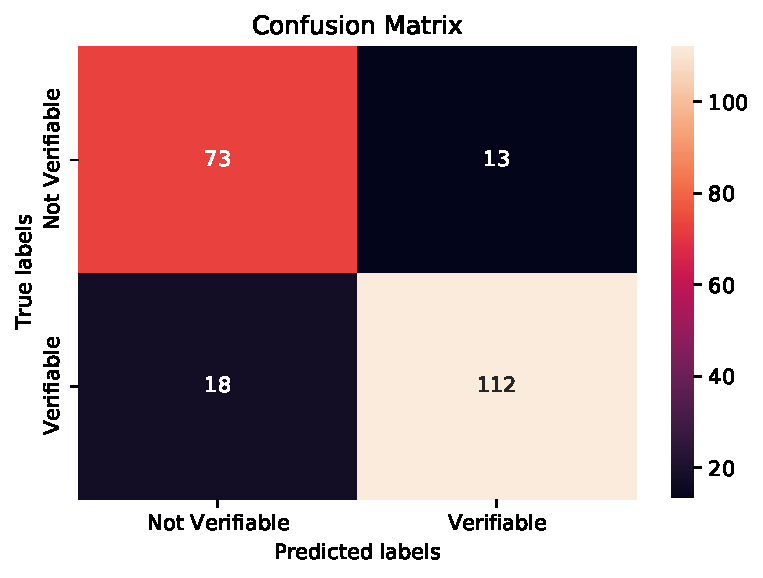
\includegraphics[width=10cm, height=9cm]{../results/desc_stats/cm_bert_2class_linear_drop3.pdf}
\end{figure}

\newpage

\subsection{Fake News Detection of Twitter and Facebook Posts Using BERT}
\label{fake_bert}

Over the years, Africa Check has manually verified thousands of posts deemed fake news and stored some of them alongside the prediction made. Out of these posts, we could recover the text from 456, which were all (except for two) classified as fake news. To add true posts and gain balance between fake and true posts, we built a data set containing around 100 thousand newspaper Tweets from the three most reliable sources in Nigeria (Mobile Punch), Kenya (Standard Kenya), and South Africa (Daily Maverick)\footnote{As recommended by the Chief Editors at AfricaCheck.}. From this 100 thousand Tweets, filtered out non-relevant Tweets related with opinions, sponsored content and business reviews and randomly sampled 30 thousand Tweets from each newspaper.\\

We further matched 456 of them to the fake ones using matching and natural language processing techniques that allowed us to identify which true post was closest to a fake one in terms of the topics they covered (identified in an automated way) and common words used in each topic.  This balanced data set, not only label-wise but also topic-wise, reduces the association between fake news and certain topics, which is usually time-dependent and affects fake news labeling outside the period of the data set. To do this we employed a LDA Topic Model\footnote{A better description of the model and the results can be found in Appendix \ref{lda_fake}}, with 5 Topics, which was fitted into the fake training data provided by Africa Check and used to predict and match on the newspaper data.

We augmented this data set with 600 political posts scraped from the FakeNet DataSet, which is a data set of US news Tweets labeled as true or fake. The label distribution of the training is in Table~\ref{tab:fake1}.

\begin{table}[ht]
\centering
\caption{Distribution of 1,518 labeled posts \label{tab:fake1}} 
\begin{tabular}{lccc}\\
  \hline
Type & Label & Number & Percent \\ 
  \hline 
\textit{Fake} & 0 & 692 & 0.456  \\ 
\textit{True} & 1 & 826 & 0.544  \\ 
   \hline
\end{tabular}
\end{table}

As with the verifiability model, after training several models using BERT, we decided on the one model which had the highest test (out of sample) accuracy, as reflected in the following confusion matrix in Figure~\ref{fig:fake2}.\\

\begin{figure}[!htpb]
    \centering
    \caption{Fake model: Confusion matrix \label{fig:fake2}}
    \label{fig:fig2}
    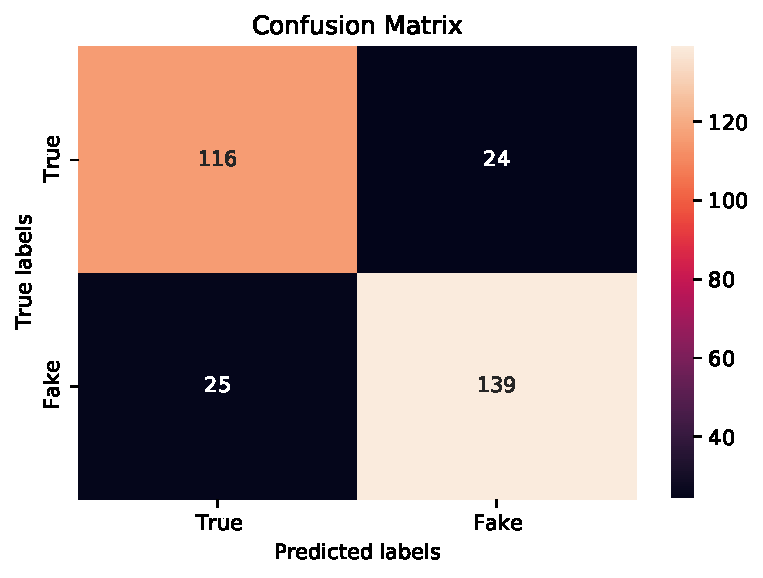
\includegraphics[width=10cm, height=8cm]{../results/desc_stats/fake_bert_linear_drop.pdf}
\end{figure}

For both models we checked the cross-validation accuracy to discard that our results were influenced by the size of our training data set and/or the sampling to split training and validation. For both cases we obtained validation accuracies close to 85$\%$, which ruled out any concern about the validity of the results.\\


\subsection{Topic modeling}

\subsubsection{LDA model: fake dataset}
\label{lda_fake}

Latent Dirichlet Allocation (LDA) is a probabilistic generative model widely employed in the field of natural language processing for topic modeling. LDA posits that documents are generated from a distribution over latent topics, with each topic characterized by a distribution of words. The model's generative process entails the assignment of topics to words in documents, guided by prior distributions \cite{Blei-LDA}\footnote{Given the timing of the deployment of the experiment, compared to when we analyzed the results of it, a few other models came into seen, like BERTopic.}. 

In our experiment, we utilized the Latent Dirichlet Allocation (LDA) model to analyze the topics present in our fake dataset. We then applied this model to predict the topics in a large collection of authentic posts gathered from reputable newspapers across Africa. After making these predictions, we compared the topic distributions of each post using a method called cosine similarity. By doing so, we were able to find the most similar authentic post for each fake post based on their topic distributions. This approach allowed us to pair each fake post with a genuine counterpart that closely matched in terms of the topics discussed.\\

We started looking at some objective measures of good fit, such as the Coherence and the Perplexity. Coherence measures the semantic similarity between high-frequency words within a topic. It helps assess how interpretable and meaningful the topics are. It is calculated by considering pairs of words that frequently co-occur within documents. A higher coherence score indicates that the words in a topic tend to be more closely related in meaning. Therefore, a good coherence score suggests that the model has successfully identified coherent topics that capture distinct themes present in the corpus \cite{CohMeasure}. On the other hand, the perplexity score measures how well the model predicts the observed documents in the dataset. A lower perplexity score indicates better predictive performance.\\

The evaluation of LDA models based solely on coherence and perplexity scores may not provide a complete understanding of which model is a better fit. As seen in Table \ref{tab:coherence}, although the scores across both dimensions are relatively similar, the model with 9 topics exhibits superior performance. However, upon closer examination of each model's relevant words, we observed that the model with 5 topics produced the most human-interpretable results. It became apparent that in models with a relatively high number of topics, there was a tendency for repeated keywords across multiple topics, indicating that the value of 'k' (the number of topics) might be too large. Furthermore, with an increase in the number of topics, their interpretability diminishes, making it more challenging to discern meaningful distinctions between them.\\

\begin{table}[H]
\caption{Topic Coherence and Perplexity across Different Models}
\centering
\label{tab:coherence}
\begin{tabular}{|c|c|c|}
\hline
Topics & Perplexity & Coherence\\
\hline
4 & -8.463 & 0.414\\
5 & -8.558 & 0.420\\
6 & -8.673 & 0.430\\
7 & -8.765 & 0.430\\
8 & -8.775 & 0.440\\
9 & -8.799 & 0.440\\
\hline
\end{tabular}
\end{table}

Given these, we decided to stick to the 5 Topic Model, since it yielded the most humanly interpretable topics. These topics, as we can see in Figure \ref{fig:LDAmodel}, are related with Economic conditions in Africa (Topic 1), Political context (Topic 2), health misinformation related with traditional medicine (Topic 3) and health misinformation related with modern medicine (Topic 5).

\begin{figure}[htbp]
    \centering
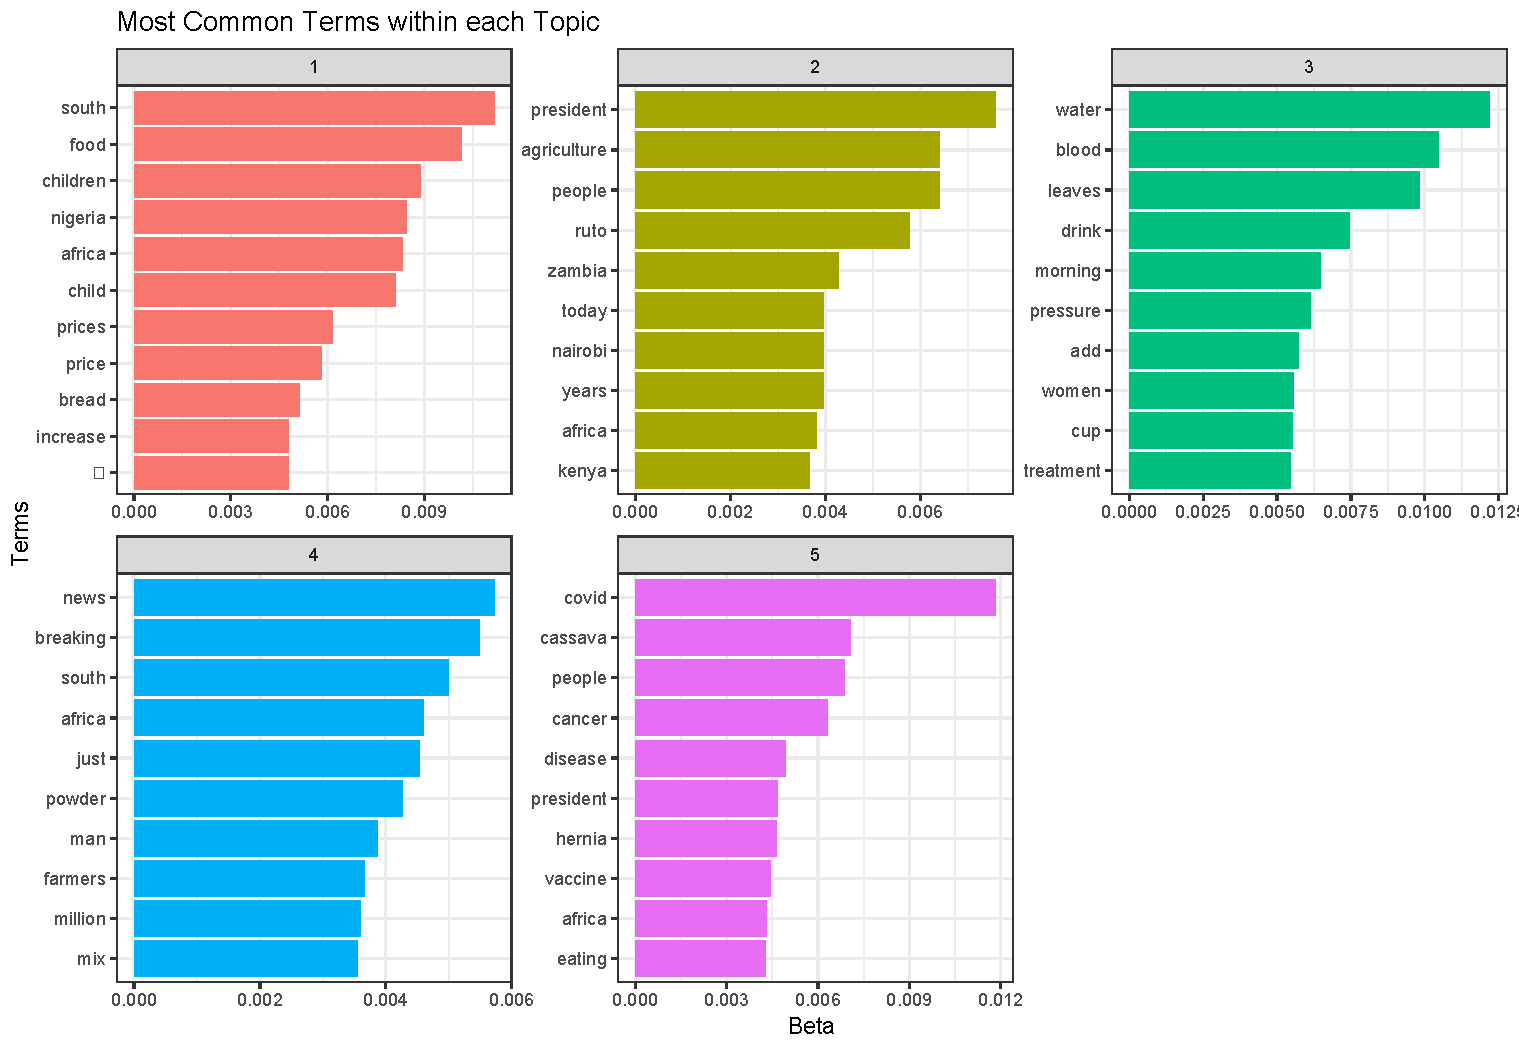
\includegraphics[width=0.98\textwidth]{../results/desc_stats/5Topics.pdf} 
        \caption{LDA Model 5 Topic Word Scores} 
    \label{fig:LDAmodel}
\end{figure}

\newpage

\subsection{COVID sentiment analysis}
\label{app:covid_bert}
Given that the information influencers posted to their followers was heavily related to COVID-19 and vaccination campaigns, an interesting outcome we analyzed was the change in sentiment towards these topics. Due to the large number of Tweets to be analyzed, we decided to use machine learning algorithms to automate the sentiment prediction of the Tweets.

We obtained a training data set from \href{https://www.kaggle.com/datasets/datatattle/covid-19-nlp-text-classification}{Kaggle}. This dataset is human-labeled and contains Tweets from all of 2020 regarding COVID-19. It has 5 labels: Extremely Positive, Positive, Neutral, Negative and Extremely Negative. For practical reasons we pooled together these 5 labels into three, Positive, Neutral and Negative. The data set is divided in training (41,157 observations) and test (3,798). Given the number of training points we have, we decided to fully balance the data set. So for our model with 3 classes we have 18,046 observations for each one of them.

For our main analysis\footnote{We also use VADER for robustness of results.}, we used a BERT (Bidirectional Encoder Representations from Transformers) model, specifically we fine-tuned the \href{https://huggingface.co/bert-base-uncased}{bert-base-uncased} and added and train a classifier layer on top of the BERT architecture. This BERT model is significantly bigger than the Small BERT (over 108 million parameters). After 5 training epochs we obtained the following metrics.

We obtained 92\% of validation accuracy and a test accuracy of 89\%, calculated by the F-Score metric. Moreover, we see no major bias in any of the classes from the confusion matrix in Figure \ref{fig:conf_BERT_base}, meaning that the model does not confuse any of the classes of has issues predicting on a particular one. Also, by looking at the learning curve in Figure \ref{fig:lc_BERT_base} we see no concern regarding over-fitting and under-fitting, which we solved through several iterations and trying different set of regularizers and even the Small BERT.

\begin{figure}[H]
    \centering
    \caption{Learning Curve: BERT Base}
    \label{fig:lc_BERT_base}
    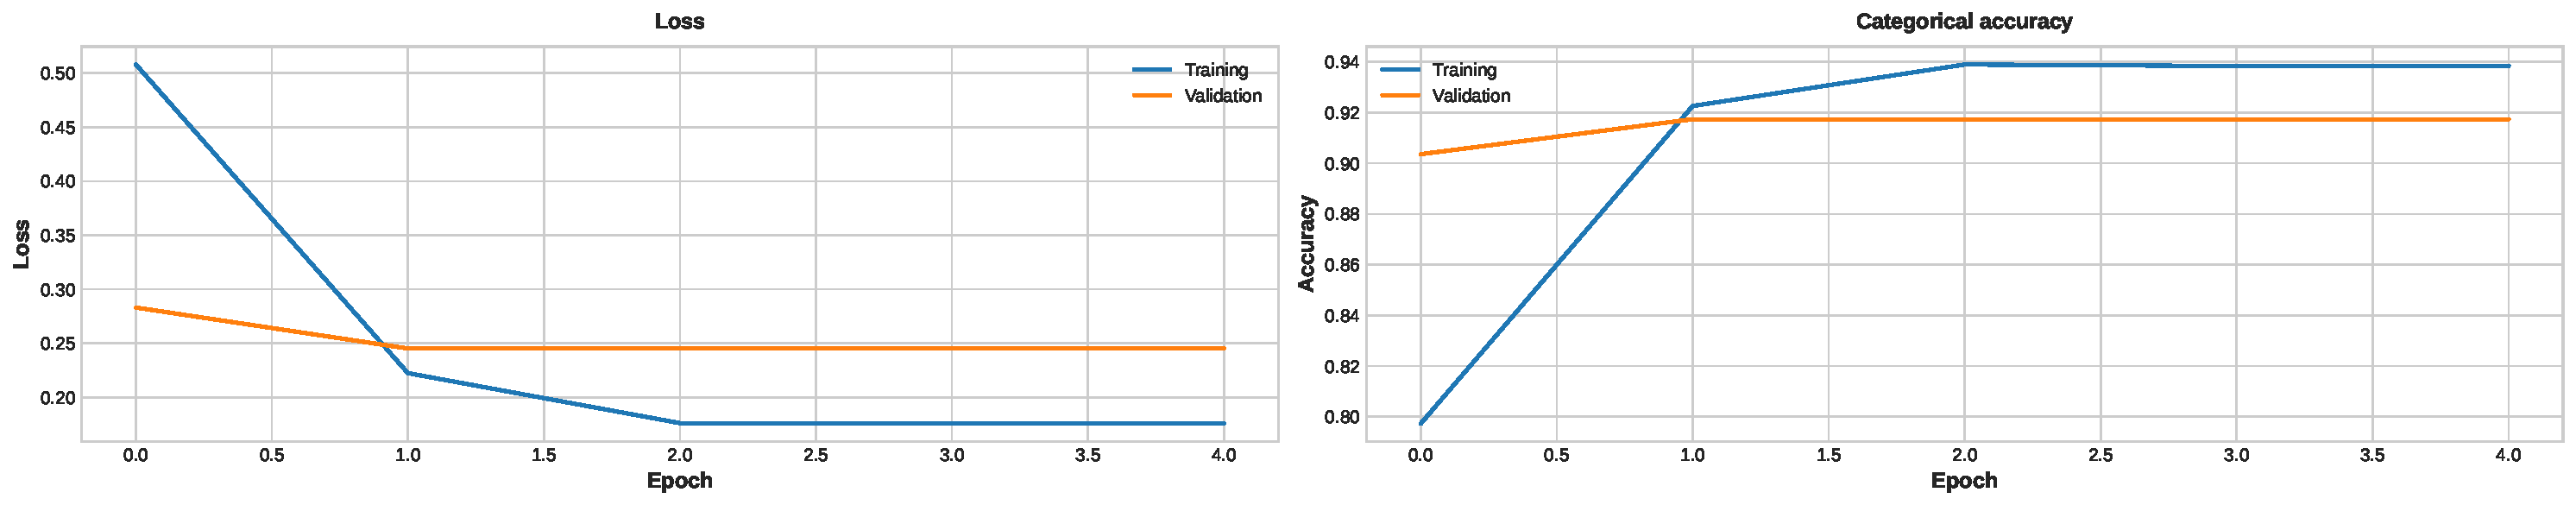
\includegraphics[width=18cm, height=9cm]{../results/desc_stats/accuracy_3classes_2.pdf}
\end{figure}

\begin{figure}[H]
    \centering
    \caption{Confusion Matrix: BERT Base}
    \label{fig:conf_BERT_base}
    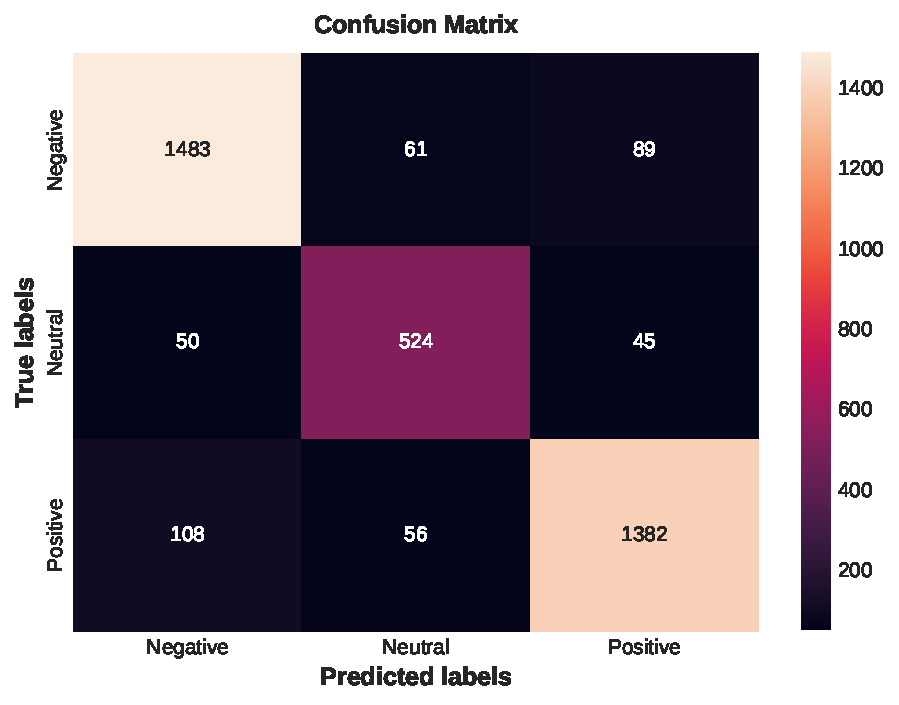
\includegraphics[width=14cm, height=10cm]{../results/desc_stats/confusion_3classes_2.pdf}
\end{figure}

\newpage


\subsection{First and Second Batch Content}
\label{app:pilot_content}
\begin{table}[ht]
		\centering
		\caption{\textbf{Africa Check Pilot Content: Kenya \label{tab:KE_1}}} 
		\begin{tabular}{|p{1cm}|p{7cm}|p{5cm}|}
			\hline
			Week & Suggested Text & Link to content \\ 
			\hline
			I & As technology advances so too has the speed and ease at which misinformation travels. To protect your friends and family, here are 5 questions to ask yourself before forwarding a message.      
            \#FactsMatter & Link: \href{https://www.dropbox.com/s/5gsfwz4tkv68q68/Africa_Check_message.mp4?dl=0}{5 Questions to Ask Before Forwarding a Message} \\ &  &\\
            I & A video shared online shows a brazen robbery and Kenyan social media users have claimed it illustrates the increase in crime in the capital Nairobi. But it’s from the South American country Guyana, not Kenya.                      
            \#FactsMatter & 
            Link: \url{https://africacheck.info/3OqcoqI}  \\ &  &\\
            II & The speed at which the Covid-19 vaccine was developed fueled understandable fears. But safety was not compromised - here’s why. \#FactsMatter & Link: \href{https://www.dropbox.com/s/qdm1q17izyxiwyl/Africa_Check_vaccine.mp4?dl=0}{The speed with which Covid-19 vaccine was developed did not compromise its safety.} \\ &  &\\
            II & Beware of Covid vaccine misinformation - a recent claim that Microsoft co-founder Bill Gates wants to “‘force-jab’ the unvaccinated” through vaccinated livestock is pure fabrication.  \#FactsMatter & Link: \url{https://africacheck.info/pfizer_employees} \\ &  &\\
            III & Seeing is believing? Not so fast. Here’s how to easily verify images and videos on social media and avoid being fooled by misinformation. \#FactsMatter & Link: \href{https://www.dropbox.com/s/kujk6fdjgasbkry/Africa_Check_youtube_image_220.mp4?dl=0}{Quick Steps to Verifying Videos or Images} \\ &  &\\
            III & A disturbing video of a girl being assaulted has been shared online with the claim the incident took place in Kenya. But the video was shot in the DRC. \#FactsMatter & Link: \url{https://africacheck.info/3RsXyBr} \\ &  &\\
            
   \hline
		\end{tabular}
  \end{table}
	\begin{table}[ht]
		\centering
  \caption{\textbf{Africa Check Content Plan: Kenya (Continued)} \label{tab:KE_2}}
		\begin{tabular}{|p{1cm}|p{7cm}|p{5cm}|}
			\hline
   IV & Heated arguments over dinner? Here’s what to do when your loved ones share misinformation, without upsetting them. \#FactsMatter & Link: \href{https://www.dropbox.com/s/s702vzeb8sc39ij/Africa_Check_misinformation.mp4?dl=0}{Dealing with family who share misinformation} \\ &  &\\
        IV & Have road crashes claimed more lives than Covid-19 in Kenya? Get the facts here:  
        \#FactsMatter
 & Link: \url{ https://africacheck.info/3jFojWA } \\ &  &\\
 V & Why do people create health disinformation? And what’s really the harm in sharing it? Keep your friends and family protected by looking out for these hidden motivations \#FactsMatter & Link: \href{https://www.dropbox.com/s/v8voe5fqa4b1fr2/Africa_Check_covid.mp4?dl=0}{Why do people share health misinformation?} \\ &  &\\
 V & While widespread antiretroviral treatment has drastically changed the lives of people with HIV, there is still no cure for the virus. Expensive treatments advertised on social media that claim otherwise should be ignored.
 \#FactsMatter
 & Link: \url{https://africacheck.info/fake_HIV_cure} \\ &  &\\
 VI & Here are @AfricaCheck’s top tips for spotting false information and stopping its spread
 \#FactsMatter & Link: \href{https://www.dropbox.com/s/wl2mzgkvqnw47dl/Africa_Check_youtube_fakenews.mp4?dl=0}{Top 4 tips to spot fake news} \\ &  &\\
 VI & A video claims that a Kenyan doctor has invented a cure for high blood pressure and is therefore in danger. The video includes the logo of KTN News and a clip of anchor Ali Manzu. But the channel – and Manzu – never reported this “news”.
 \#FactsMatter
 & Link: \url{https://africacheck.info/3WY6twP} \\ &  &\\
\hline
		\end{tabular}
\end{table}


	\begin{table}[ht]
		\centering
  \caption{\textbf{Africa Check Content Plan: Kenya  (Continued)} \label{tab:KE_3}}
		\begin{tabular}{|p{1cm}|p{7cm}|p{5cm}|}
			\hline
   VII & Medical advice and health tips are everywhere on social media. But some aren’t backed by science, and can even cause harm. These verification steps can help protect family and friends from health
misinformation
 \#FactsMatter & Link: \href{https://www.dropbox.com/s/b2bxkbjwtzp2xnr/Africa_Check_health.mp4?dl=0}{Verifying health claims quacks or false cures} \\ &  &\\
 VII & Some substances extracted from pineapples may help treat less serious conditions. But “hot pineapple water” definitely doesn’t cure cancer. This dangerous claim rehashes old (untrue) advice that “hot lemon water” cures cancer. \#FactsMatter
 & Link: \url{https://africacheck.info/3kGLAIe} \\ &  &\\
 VIII & IT’S A SCAM! Make sure you’re not fooled by using these simple steps.
 \#FactsMatter & Link: \href{https://www.dropbox.com/s/9gvyb2x4j09thiv/Africa_Check_facebook.mp4?dl=0}{Facebook scams and how to stop them} \\ &  &\\
 VIII & Beware of posts offering soft loans on WhatsApp from Kenya’s Family Bank. The loan terms are attractive. But the offer isn’t real, confirming that if something sounds too good to be true, it usually is. \#FactsMatter
 & Link: \url{https://africacheck.info/3lx7cHt} \\ &  &\\
\hline 
   \end{tabular}
\end{table}

\newpage

\begin{table}[ht]
		\centering
		\caption{\textbf{Africa Check First and Second Batch Content: South Africa \label{tab:SA_1}}} 
		\begin{tabular}{|p{1cm}|p{7cm}|p{5cm}|}
			\hline
			Week & Suggested Text & Link to content \\ 
			\hline
			I & As technology advances so too has the speed and ease at which misinformation travels. To protect your friends and family, here are 5 questions to ask yourself before forwarding a message.      
            \#FactsMatter & Link: \href{https://www.dropbox.com/s/5gsfwz4tkv68q68/Africa_Check_message.mp4?dl=0}{5 Questions to Ask Before Forwarding a Message} \\ &  &\\
            I & What do we know about race and private sector ownership in South Africa? Three viral claims are investigated here: 
            \#FactsMatter & 
            Link: \url{https://africacheck.info/3B86Trx} \\ &  &\\
            II & The speed at which the Covid-19 vaccine was developed fueled understandable fears. But safety was not compromised - here’s why. \#FactsMatter & Link: \href{https://www.dropbox.com/s/qdm1q17izyxiwyl/Africa_Check_vaccine.mp4?dl=0}{The speed with which Covid-19 vaccine was developed did not compromise its safety.} \\ &  &\\
            II & A claim that South Africans were given the “wrong Covid vaccine” is incorrect. A batch of nasal spray to help treat Covid symptoms was ordered by the defence department, but returned to Cuba after the public protector stepped in. \#FactsMatter & Link: \url{https://africacheck.info/3W19A6K} \\ &  &\\
            III & Seeing is believing? Not so fast. Here’s how to easily verify images and videos on social media and avoid being fooled by misinformation. \#FactsMatter & \href{https://www.dropbox.com/s/kujk6fdjgasbkry/Africa_Check_youtube_image_220.mp4?dl=0}{Quick Steps to Verifying Videos or Images} \\ &  &\\
            III & No, this photo doesn't show the British ambassador to Somalia with a black child in a cage.  \#FactsMatter & Link: \url{https://africacheck.info/british_ambassador_somalia} \\ &  &\\
            
   \hline
		\end{tabular}
  \end{table}

  
	\begin{table}[ht]
		\centering
     \caption{\textbf{Africa Check Content Plan: South Africa (Continued)} \label{tab:SA_2}}
		\begin{tabular}{|p{1cm}|p{7cm}|p{5cm}|}
			\hline
   IV & Heated arguments over dinner? Here’s what to do when your loved ones share misinformation, without upsetting them. \#FactsMatter & Link: \href{https://www.dropbox.com/s/s702vzeb8sc39ij/Africa_Check_misinformation.mp4?dl=0}{Dealing with family who share misinformation} \\ &  &\\
        IV & Is \#SouthAfrica’s much-criticised power utility @Eskom\_SA overstaffed by 66\%? And do salaries for 27,543 surplus staff amount to R1.38 billion per year? 
        These claims have been much shared online. But are they accurate? 
        \#FactsMatter
 & Link: \url{https://africacheck.info/eskom_salaries} \\ &  &\\
 V & Why do people create health disinformation? And what’s really the harm in sharing it? Keep your friends and family protected by looking out for these hidden motivations \#FactsMatter & Link: \href{https://www.dropbox.com/s/v8voe5fqa4b1fr2/Africa_Check_covid.mp4?dl=0}{Why do people share health misinformation?} \\ &  &\\
 V & While widespread antiretroviral treatment has drastically changed the lives of people with HIV, there is still no cure for the virus. Expensive treatments advertised on social media that claim otherwise should be ignored. \#FactsMatter
 & Link: \url{https://africacheck.info/fake_HIV_cure} \\ &  &\\
 VI & Here are @AfricaCheck’s top tips for spotting false information and stopping its spread
 \#FactsMatter & Link: \href{https://www.dropbox.com/s/wl2mzgkvqnw47dl/Africa_Check_youtube_fakenews.mp4?dl=0}{Top 4 tips to spot fake news} \\ &  &\\
 VI & Government ministers do sometimes put their feet in their mouths. But there’s no evidence South African minister of water \& sanitation suggested people shower ‘in groups’, however dire the country’s water and electricity crises might be.
 \#FactsMatter
 & Link: \url{https://africacheck.info/3U7Flt3} \\ &  &\\
\hline
		\end{tabular}
  \end{table}

  
	\begin{table}[ht]
		\centering
  \caption{\textbf{Africa Check Content Plan: South Africa (Continued)} \label{tab:SA_3}}
		\begin{tabular}{|p{1cm}|p{7cm}|p{5cm}|}
			\hline
   VII & Medical advice and health tips are everywhere on social media. But some aren’t backed by science, and can even cause harm. These verification steps can help protect family and friends from health
misinformation
 \#FactsMatter & Link: \href{https://www.dropbox.com/s/b2bxkbjwtzp2xnr/Africa_Check_health.mp4?dl=0}{Verifying health claims quacks or false cures} \\ &  &\\
 VII & Some substances extracted from pineapples may help treat less serious conditions. But “hot pineapple water” definitely doesn’t cure cancer. This dangerous claim rehashes old (untrue) advice that “hot lemon water” cures cancer.
  \#FactsMatter & Link: \url{https://africacheck.info/3kGLAIe} \\ &  &\\
 VIII & IT'S A SCAM! Make sure you're not fooled by using these simple steps.
 \#FactsMatter & Link: \href{https://www.dropbox.com/s/9gvyb2x4j09thiv/Africa_Check_facebook.mp4?dl=0}{Facebook scams and how to stop them} \\ &  &\\
 VIII & Beware of rings sold with the promise of weight loss or health benefits. It’s a scam, confirming that if something sounds too good to be true, it usually is.
  \#FactsMatter
 & Link: \url{https://africacheck.info/3wphJGV} \\ &  &\\
\hline 
   \end{tabular}
\end{table}



\end{document}
